\section{Tests and Results}
\label{sec:testsResults}
	\subsection{Procedure 1}
		\label{sec:testsResults:subsec:Experimento01}
		\par The tests, and corresponding results, for already described procedure 1   are found in this section. As explained in that opportunity, this procedure aims, based on Paraconsistent Engineering, to find which \textit{wavelet} filter provides, together with the Bark or Mel scale, the shortest distance from the point $(G_1,G_2)$ to the vertex $(1,0)$ of the paraconsistent plane.\\
		
		\par Particularly, in Figure \ref{fig:paraconsistentfull}, which combines the results of the filters with the scales, the shorter the horizontal length of the bars in blue, the better the separability between the classes. As can be seen, from the tested combinations, \textbf{Haar+Bark} provided the shortest distance. In addition, the tables \ref{tab:distParacomFrom10Bark_1}, \ref{tab:distParacomFrom10Bark_2}, \ref{tab:distParacomFrom10Mel_1} and \ref{tab:distParacomFrom10Mel_2} contains the specific values displayed graphically in that Figure.\\
		
		\par The \textbf{\textit{wavelet}+Bark} combination consistently presented \textbf{better} viability than the respective combinations of \textbf{\textit{wavelet+Mel}}.\\
		
		\par Analyzing the behavior of the best and worst \textit{wavelets} found, it is interesting to ask why the \textbf{Haar} filters have provided the best results. Particularly interesting is the fact that the \textit{wavelet} filters of \textbf{Haar} and \textbf{Daubechies 42} provided, respectively, the best and worst results associated with the Bark scale. In contrast, with the \textit{Mel} scale, \textbf{Haar} was the best filter and \textbf{Daubechies 54} the worst.)\\

		\par Dicussing about the phase and frequency response characteristics of the \textit{wavelet} filters, we can see the following: Haar presents the frequency response curve that is the most distant from the ideal, as it constitutes a finite impulse response filter (FIR) of order 1, that is, with two coefficients \cite{WaveletPropertiesBrowser}. Therefore, specific frequency sub-bands are undoubtedly contaminated with spectral content from adjacent sub-bands. Additionally, Haar is the only family of \textit{wavelet} filters that has a perfectly linear phase response. So, from the filters point of view, what has been verified experimentally is that a non-rigorous frequency response associated with a perfectly linear phase response is the best alternative.)

		\begin{center}
	\newcommand{\mc}[3]{\multicolumn{#1}{#2}{#3}}
	\definecolor{tcB}{rgb}{0.447059,0.74902,0.266667}
	\definecolor{tcA}{rgb}{0.65098,0.65098,0.65098}
	\definecolor{tcC}{rgb}{0,0.8,1}
	
	\begin{longtable}[h]{|c|c|c|c|c|}
		
		% Columns headers
		\hline
		\mc{1}{|>{\columncolor{tcA}}c|}{Mel/Bark}&\mc{1}{|>{\columncolor{tcA}}c|}{Wavelet}&\mc{1}{|>{\columncolor{tcA}}c|}{G1}&\mc{1}{|>{\columncolor{tcA}}c|}{G2}&\mc{1}{|>{\columncolor{tcA}}c|}{Distância de (1,0)}\\\hline
		\endfirsthead
		
		\mc{3}{c}{{\tablename\ \thetable : Continuação da página anterior}} \\\hline
		% Columns headers
		\mc{1}{|>{\columncolor{tcA}}c|}{Mel/Bark}&\mc{1}{|>{\columncolor{tcA}}c|}{Wavelet}&\mc{1}{|>{\columncolor{tcA}}c|}{G1}&\mc{1}{|>{\columncolor{tcA}}c|}{G2}&\mc{1}{|>{\columncolor{tcA}}c|}{Distance to (1,0)}\\\hline
		\endhead
		
		\hline \mc{2}{c}{{Continua na próxima página}} \\
		\endfoot
		\endlastfoot
		
		% Color of the first line
		\rowcolor{tcB}
		
		% Loads data from tables/results/paraconsistentPlane/distParacomFrom10.csv
		\csvreader[
		no head,
		late after line=\\\hline\rowcolor{tcC},%
		separator=comma,
		filter={\value{csvrow}<4},
		]{../monography/tables/results/paraconsistentPlane/distParacomFrom10.csv}{
			1=\melBark,
			2=\wavelet,
			3=\gOne,
			4=\gTwo,
			5=\distance
		}{
			\melBark&
			\wavelet&
			\StrSubstitute[0]{\gOne}{.}{,}&
			\StrSubstitute[0]{\gTwo}{.}{,}&
			\StrSubstitute[0]{\distance}{.}{,}
		}
		
		\rowcolor{white}
		\caption{As 5 primeiras combinações Wavelet \textit{x} Mel/Bark ordenadas pela distância do vértice (1,0) no plano paraconsistente.}
		\label{tab:distParacomFrom10BarkAndMel}
	\end{longtable}
\end{center}
		
		\clearpage
		\begin{figure}[H]
			\centering
			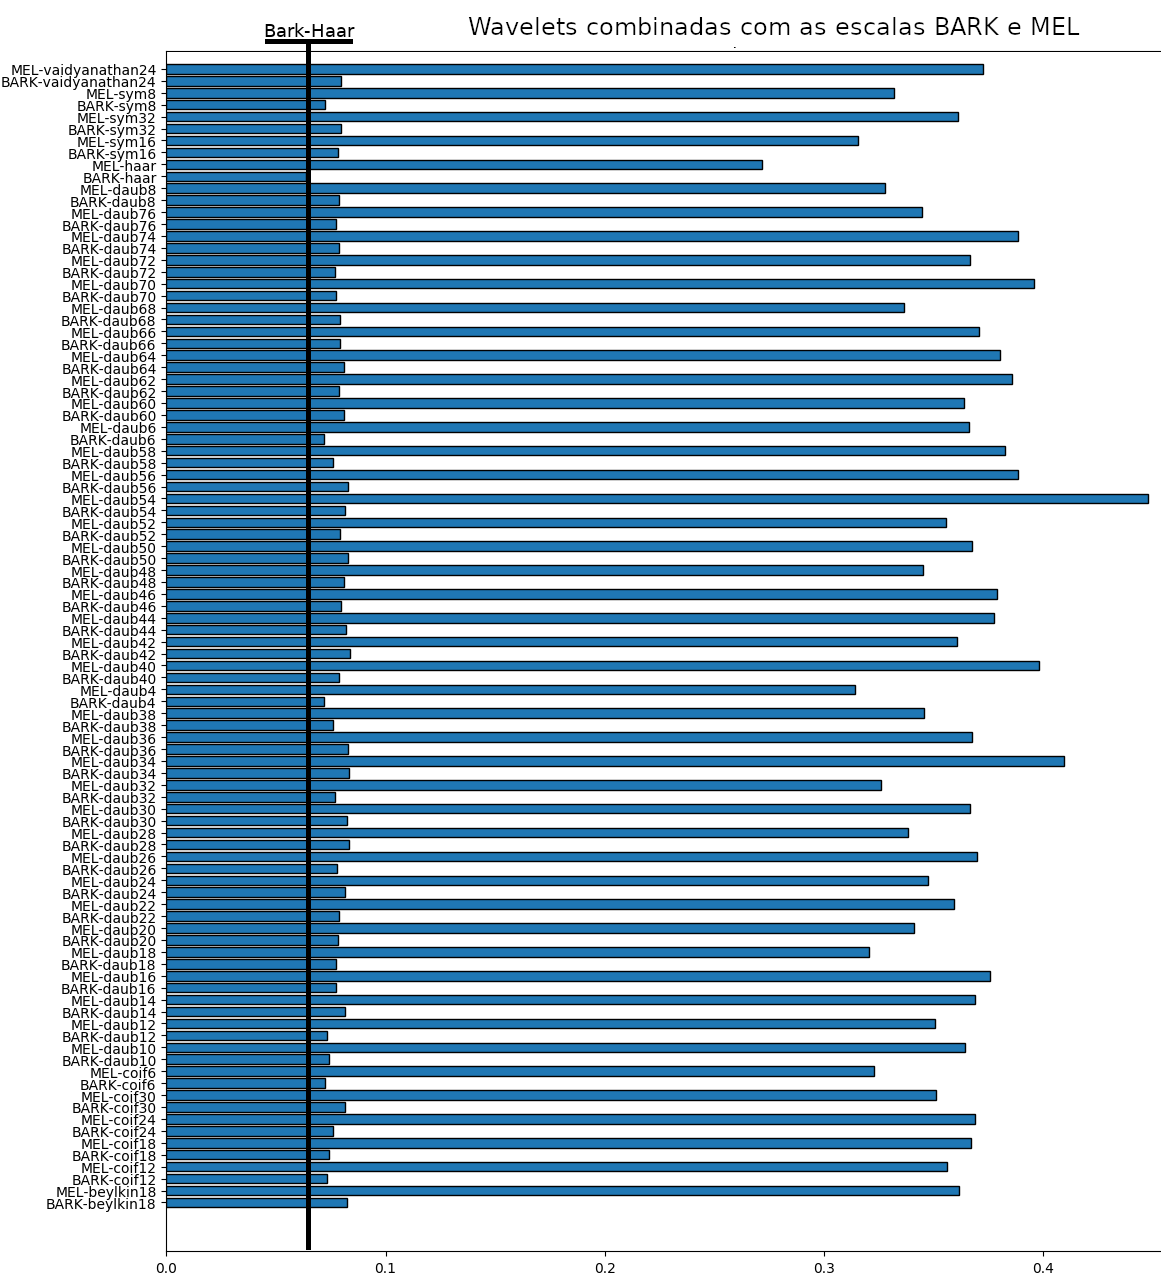
\includegraphics[width=0.99\linewidth]{images/results/paraconsistentPlane/ParaconsistentFull.png}
			\caption{Gráfico completo da distância ao ponto (1,0) no plano paraconsistente.}
			\label{fig:paraconsistentfull}
		\end{figure}
		
		\par From the point of view of the Bark and Mel bands, Bark is, according to the comments in Chapter 2, the one that was more broadly defined to reflect the behavior of human hearing for acoustic signals in general. Unlike Mel band, which was optimized for voice but, according to the experiments, it did not provide the best results. Therefore, it is clear that the \textbf{noisy characteristic} of the spoofed signals, containing, unlike the original voices, notorious components of high frequencies, is better detected with a scale more appropriate to the treatment of audio in general and not only voice.)
		
		
	\subsection{Procedure 2} 
		\label{sec:testsResults:subsec:Experimento02}
		\par Considering that, according to procedure 01, the best result was the combination \textbf{Haar + Bark}, the objective of this procedure is \textbf{to verify the maximum accuracy and the minimum EER} that can be achieved with the use of a classifier based on Euclidean and Manhattan distances, according to the details defined in the previous Chapter.\\
		
		\par Therefore, for the amounts of 10\%, 20\%, 30\%, 40\% and 50\% of the signals in database reserved for training, with the limit of 300 random tests in each case, the results obtained are shown in Tables \ref{tab: experiment02ResultsEuclidian} and \ref{tab:experiment02ResultsManhattan}. Particularly interesting in them, is the measure of the equal error rate (EER), which balances the rates of false positives and false negatives.
		\\
		
		\par Further details for the Euclidean distance can be obtained by consulting the Tables
		 \ref{tab:classifier_Euclidian_10_best}, \ref{tab:classifier_Euclidian_10_worse},
		\ref{tab:classifier_Euclidian_20_best}, \ref{tab:classifier_Euclidian_20_worse}, 
		\ref{tab:classifier_Euclidian_30_best}, \ref{tab:classifier_Euclidian_30_worse}, 
		\ref{tab:classifier_Euclidian_40_best}, \ref{tab:classifier_Euclidian_40_worse}, 
		\ref{tab:classifier_Euclidian_50_best}, \ref{tab:classifier_Euclidian_50_worse}
		and its respective graphs in the Figures \ref{fig:classifiereuclidian10}, \ref{fig:classifiereuclidian20}, \ref{fig:classifiereuclidian30}, \ref{fig:classifiereuclidian40} e \ref{fig:classifiereuclidian50}. For Manhattan distances, the tables \ref{tab:classifier_Manhattan_10_best}, \ref{tab:classifier_Manhattan_10_worst}, 
		\ref{tab:classifier_Manhattan_20_best}, \ref{tab:classifier_Manhattan_20_worst}, 
		\ref{tab:classifier_Manhattan_30_best}, \ref{tab:classifier_Manhattan_30_worse}, 
		\ref{tab:classifier_Manhattan_40_best}, \ref{tab:classifier_Manhattan_40_worse}, 
		\ref{tab:classifier_Manhattan_50_best}, \ref{tab:classifier_Manhattan_50_worse} 
		can be consulted toguether with its respective graphs \ref{fig:classifiermanhattan10}, \ref{fig:classifiermanhattan20}, \ref{fig:classifiermanhattan30}, \ref{fig:classifiermanhattan40}, \ref{fig:classifiermanhattan50}.\\
		
		\begin{table}[h]
	\newcommand{\mc}[3]{\multicolumn{#1}{#2}{#3}}
	\definecolor{tcA}{rgb}{0.65098,0.65098,0.65098}
	\definecolor{tcB}{rgb}{0.447059,0.74902,0.266667}
	\begin{center}
		\begin{tabular}{|l|l|l|}\hline
			% use packages: color,colortbl
			\rowcolor{tcA}
			\textbf{Tamanho do modelo} & \textbf{Acurácia mínima} & \textbf{Acurácia máxima}\\\hline
			\rowcolor{tcB}
			\mc{1}{|c|}{10\%} & \mc{1}{c|}{0,6666} & \mc{1}{c|}{0,8861}\\\hline
			\rowcolor{tcB}
			\mc{1}{|c|}{20\%} & \mc{1}{c|}{0,7439} & \mc{1}{c|}{0,8902}\\\hline
			\rowcolor{tcB}
			\mc{1}{|c|}{30\%} & \mc{1}{c|}{0,7665} & \mc{1}{c|}{0,8919}\\\hline
			\rowcolor{tcB}
			\mc{1}{|c|}{40\%} & \mc{1}{c|}{0,7784} & \mc{1}{c|}{0,9024}\\\hline
			\rowcolor{tcB}
			\mc{1}{|c|}{50\%} & \mc{1}{c|}{0,7804} & \mc{1}{c|}{0,9097}\\\hline
		\end{tabular}
	\end{center}
	\caption{Resultados do experimento 02}
	\label{tab:experiment02Results}
\end{table}

		\subsubsection{BARK scale with Haar \textit{wavelet} using an Euclidean distance classifier at 10\% model}
		
			\begin{table}[H] 					\newcommand{\mc}[3]{\multicolumn{#1}{#2}{#3}} 					\definecolor{tcB}{rgb}{0.447059,0.74902,0.266667} 					\definecolor{tcC}{rgb}{0,0,0} 					\definecolor{tcD}{rgb}{0,0.5,1} 					\definecolor{tcA}{rgb}{0.65098,0.65098,0.65098} 					\begin{center} 						\subfloat[Melhor matriz de confusão]{ 							\begin{tabular}{ccc} 								\mc{1}{l}{} & \mc{1}{>{\columncolor{tcA}}c}{\textbf{genuíno}} & \mc{1}{>{\columncolor{tcA}}c}{\textbf{falseado}}\\ 								\mc{1}{>{\columncolor{tcA}}r}{\textbf{genuíno}} & \mc{1}{>{\columncolor{tcB}}c}{\textcolor{tcC}{363}} & \mc{1}{>{\columncolor{tcD}}c}{\textcolor{tcC}{14}}\\ 								\mc{1}{>{\columncolor{tcA}}r}{\textbf{falseado}} & \mc{1}{>{\columncolor{tcD}}c}{\textcolor{tcC}{6}} & \mc{1}{>{\columncolor{tcB}}c}{\textcolor{tcC}{355}} 							\end{tabular} 							\label{tab:classifier_Euclidian_10_best} 						} 						\qquad 						\subfloat[Pior matriz de confusão]{ 							\begin{tabular}{ccc} 								\mc{1}{l}{} & \mc{1}{>{\columncolor{tcA}}c}{\textbf{genuíno}} & \mc{1}{>{\columncolor{tcA}}c}{\textbf{falseado}}\\ 								\mc{1}{>{\columncolor{tcA}}r}{\textbf{genuíno}} & \mc{1}{>{\columncolor{tcB}}c}{\textcolor{tcC}{275}} & \mc{1}{>{\columncolor{tcD}}c}{\textcolor{tcC}{10}}\\ 								\mc{1}{>{\columncolor{tcA}}r}{\textbf{falseado}} & \mc{1}{>{\columncolor{tcD}}c}{\textcolor{tcC}{94}} & \mc{1}{>{\columncolor{tcB}}c}{\textcolor{tcC}{359}} 							\end{tabular} 							\label{tab:classifier_Euclidian_10_worse} 						} 					\end{center} 					\caption{Matrizes de confusão para distância Euclidiana com modelo a 10\%} 				\end{table}
			
			\begin{figure}[!h]
				\centering
				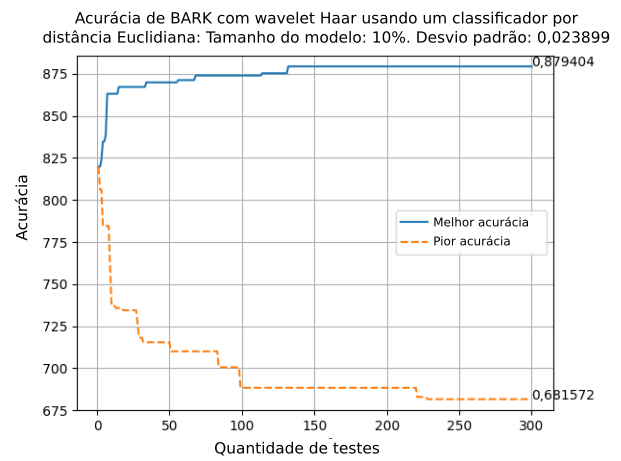
\includegraphics[width=\linewidth]{images/results/confusionMatrices/classifier_Euclidian_10}
				\caption{Accuracy \textit{X} number of tests - Euclidean distance, model at 10\%}
				\label{fig:classifiereuclidian10}
			\end{figure}
			
			\begin{figure}[!h]
				\centering
				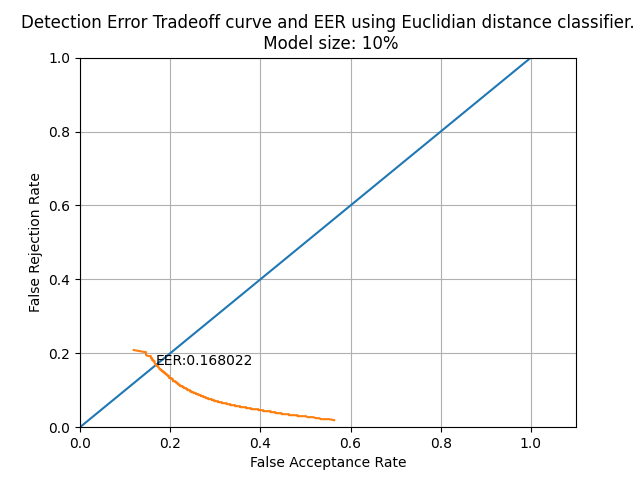
\includegraphics[width=.9\linewidth]{images/results/det/DET_for_classifier_Euclidian_10}
				\caption{DET curve of Euclidean distance results, model at 10\% }
				\label{fig:detforclassifiereuclidian10}
			\end{figure}
		
		\subsubsection{BARK scale with Haar \textit{wavelet} using an Euclidean distance classifier at 20\% model}
		
			\begin{table}[h]
\newcommand{\mc}[3]{\multicolumn{#1}{#2}{#3}}
\definecolor{tcB}{rgb}{0.447059,0.74902,0.266667}
\definecolor{tcC}{rgb}{0,0,0}
\definecolor{tcD}{rgb}{0,0.4,0.701961}
\definecolor{tcA}{rgb}{0.65098,0.65098,0.65098}
\begin{center}
	\begin{tabular}{ccc}
		% use packages: color,colortbl
		\mc{1}{l}{} & \mc{1}{>{\columncolor{tcA}}c}{\textbf{genuíno}} & \mc{1}{>{\columncolor{tcA}}c}{\textbf{regravado}}\\

		\mc{1}{>{\columncolor{tcA}}r}{\textbf{genuíno}} & \mc{1}{>{\columncolor{tcB}}c}{\textcolor{tcC}{308}} & \mc{1}{>{\columncolor{tcD}}c}{\textcolor{tcC}{50}}\\

		\mc{1}{>{\columncolor{tcA}}r}{\textbf{regravado}} & \mc{1}{>{\columncolor{tcD}}c}{\textcolor{tcC}{20}} & \mc{1}{>{\columncolor{tcB}}c}{\textcolor{tcC}{278}}
	\end{tabular}
	\caption{Melhor matriz de confusão para o classificador por distâncias Euclidianas com o uso de 20\% da base para modelagem}
	\label{tab:classifier_Euclidian_20_best}
\end{center}
\end{table}

\begin{table}[h]
	\newcommand{\mc}[3]{\multicolumn{#1}{#2}{#3}}
	\definecolor{tcB}{rgb}{0.447059,0.74902,0.266667}
	\definecolor{tcC}{rgb}{0,0,0}
	\definecolor{tcD}{rgb}{0,0.4,0.701961}
	\definecolor{tcA}{rgb}{0.65098,0.65098,0.65098}
	\begin{center}
		\begin{tabular}{ccc}
			% use packages: color,colortbl
			\mc{1}{l}{} & \mc{1}{>{\columncolor{tcA}}c}{\textbf{genuíno}} & \mc{1}{>{\columncolor{tcA}}c}{\textbf{regravado}}\\
			
			\mc{1}{>{\columncolor{tcA}}r}{\textbf{genuíno}} & \mc{1}{>{\columncolor{tcB}}c}{\textcolor{tcC}{295}} & \mc{1}{>{\columncolor{tcD}}c}{\textcolor{tcC}{137}}\\
			
			\mc{1}{>{\columncolor{tcA}}r}{\textbf{regravado}} & \mc{1}{>{\columncolor{tcD}}c}{\textcolor{tcC}{33}} & \mc{1}{>{\columncolor{tcB}}c}{\textcolor{tcC}{191}}
		\end{tabular}
		\caption{Pior matriz de confusão para o classificador por distâncias Euclidianas com o uso de 20\% da base para modelagem}
		\label{tab:classifier_Euclidian_20_worse}
	\end{center}
\end{table}

			
			\begin{figure}[ht]
				\centering
				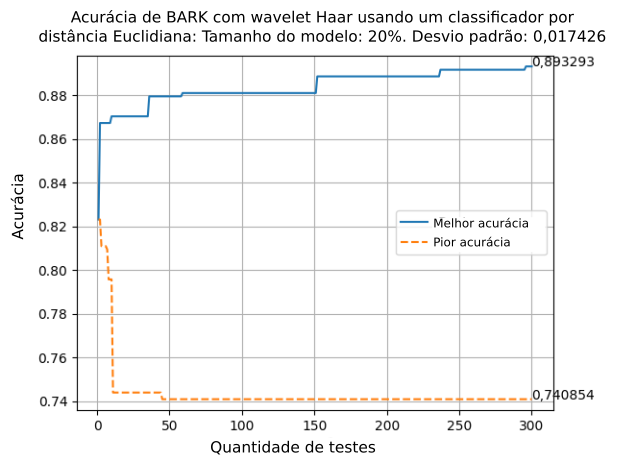
\includegraphics[width=\linewidth]{images/results/confusionMatrices/classifier_Euclidian_20}
				\caption{Accuracy \textit {X} number of tests - Euclidean distance, model at 20\%}
				\label{fig:classifiereuclidian20}
			\end{figure}
			
			\begin{figure}[!ht]
				\centering
				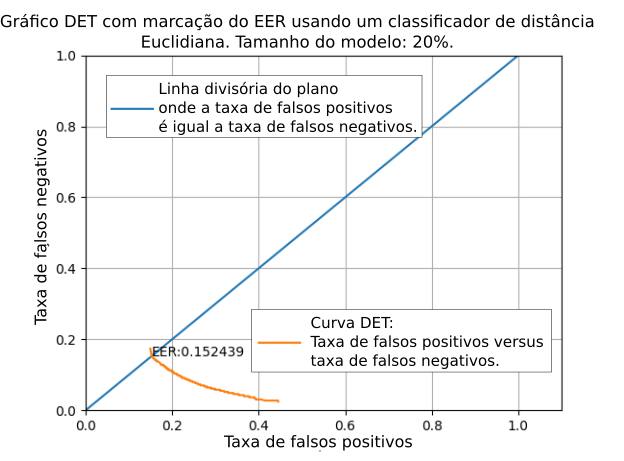
\includegraphics[width=.9\linewidth]{images/results/det/DET_for_classifier_Euclidian_20}
				\caption{DET curve of Euclidean distance results, model at 10\%}
				\label{fig:detforclassifiereuclidian20}
			\end{figure}
		
		\subsubsection{BARK scale with Haar \textit{wavelet} using an Euclidean distance classifier at 30\% model}
		
			\begin{table}[H] 					\newcommand{\mc}[3]{\multicolumn{#1}{#2}{#3}} 					\definecolor{tcB}{rgb}{0.447059,0.74902,0.266667} 					\definecolor{tcC}{rgb}{0,0,0} 					\definecolor{tcD}{rgb}{0,0.5,1} 					\definecolor{tcA}{rgb}{0.65098,0.65098,0.65098} 					\begin{center} 		\caption{Matrizes de confusão para distância Euclidiana com modelo a 30\%}				\subfloat[Melhor matriz de confusão]{ 							\begin{tabular}{ccc} 								\mc{1}{l}{} & \mc{1}{>{\columncolor{tcA}}c}{\textbf{genuíno}} & \mc{1}{>{\columncolor{tcA}}c}{\textbf{falseado}}\\ 								\mc{1}{>{\columncolor{tcA}}r}{\textbf{genuíno}} & \mc{1}{>{\columncolor{tcB}}c}{\textcolor{tcC}{283}} & \mc{1}{>{\columncolor{tcD}}c}{\textcolor{tcC}{8}}\\ 								\mc{1}{>{\columncolor{tcA}}r}{\textbf{falseado}} & \mc{1}{>{\columncolor{tcD}}c}{\textcolor{tcC}{4}} & \mc{1}{>{\columncolor{tcB}}c}{\textcolor{tcC}{279}} 							\end{tabular} 							\label{tab:classifier_Euclidian_30_best} 						} 						\qquad 						\subfloat[Pior matriz de confusão]{ 							\begin{tabular}{ccc} 								\mc{1}{l}{} & \mc{1}{>{\columncolor{tcA}}c}{\textbf{genuíno}} & \mc{1}{>{\columncolor{tcA}}c}{\textbf{falseado}}\\ 								\mc{1}{>{\columncolor{tcA}}r}{\textbf{genuíno}} & \mc{1}{>{\columncolor{tcB}}c}{\textcolor{tcC}{258}} & \mc{1}{>{\columncolor{tcD}}c}{\textcolor{tcC}{20}}\\ 								\mc{1}{>{\columncolor{tcA}}r}{\textbf{falseado}} & \mc{1}{>{\columncolor{tcD}}c}{\textcolor{tcC}{29}} & \mc{1}{>{\columncolor{tcB}}c}{\textcolor{tcC}{267}} 							\end{tabular} 							\label{tab:classifier_Euclidian_30_worse} 						} 					\\Fonte: Elaborado pelo autor, 2021.		\end{center} 					 				\end{table}
			
			\begin{figure}[ht]
				\centering
				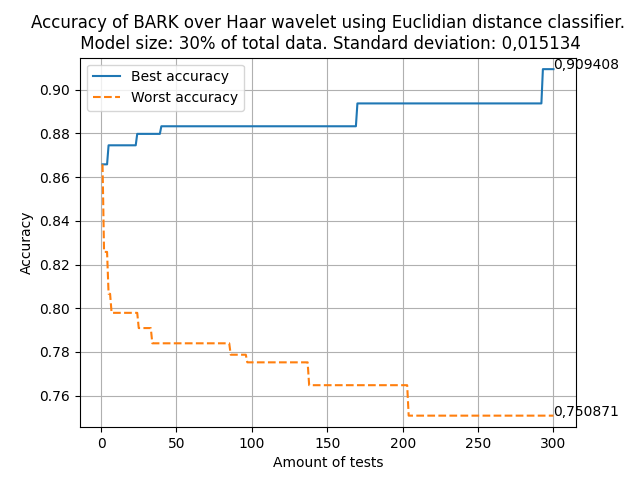
\includegraphics[width=\linewidth]{images/results/confusionMatrices/classifier_Euclidian_30}
				\caption{Accuracy \textit{X} number of tests - Euclidean distance, model at 30\%}
				\label{fig:classifiereuclidian30}
			\end{figure}
			
			\begin{figure}[ht]
				\centering
				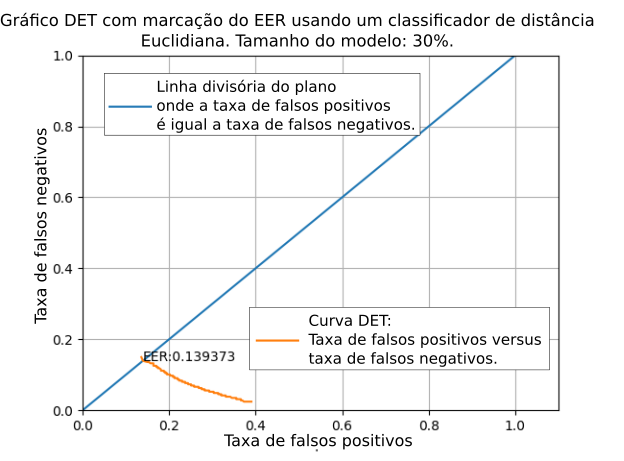
\includegraphics[width=.9\linewidth]{images/results/det/DET_for_classifier_Euclidian_30}
				\caption{DET curve of Euclidean distance results, model at 30\%}
				\label{fig:detforclassifiereuclidian30}
			\end{figure}
		
		\subsubsection{BARK scale with Haar \textit{wavelet} using an Euclidean distance classifier at 40\% model}
		
			\begin{table}[h]
\newcommand{\mc}[3]{\multicolumn{#1}{#2}{#3}}
\definecolor{tcB}{rgb}{0.447059,0.74902,0.266667}
\definecolor{tcC}{rgb}{0,0,0}
\definecolor{tcD}{rgb}{0,0.4,0.701961}
\definecolor{tcA}{rgb}{0.65098,0.65098,0.65098}
\begin{center}
	\begin{tabular}{ccc}
		% use packages: color,colortbl
		\mc{1}{l}{} & \mc{1}{>{\columncolor{tcA}}c}{\textbf{Verdadeiro}} & \mc{1}{>{\columncolor{tcA}}c}{\textbf{Falso}}\\

		\mc{1}{>{\columncolor{tcA}}r}{\textbf{Verdadeiro}} & \mc{1}{>{\columncolor{tcB}}c}{\textcolor{tcC}{233}} & \mc{1}{>{\columncolor{tcD}}c}{\textcolor{tcC}{35}}\\

		\mc{1}{>{\columncolor{tcA}}r}{\textbf{Falso}} & \mc{1}{>{\columncolor{tcD}}c}{\textcolor{tcC}{13}} & \mc{1}{>{\columncolor{tcB}}c}{\textcolor{tcC}{211}}
	\end{tabular}
	\caption{Tabela de confusão para classificador Euclidiano 40\%}
	\label{tab:classifier_Euclidian_40}
\end{center}
\end{table}

			
			\begin{figure}[ht]
				\centering
				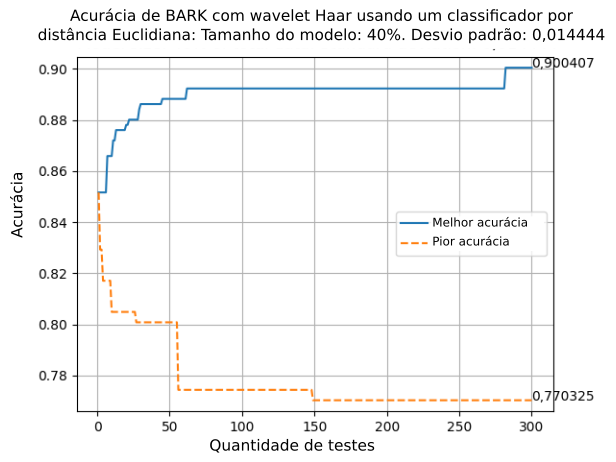
\includegraphics[width=\linewidth]{images/results/confusionMatrices/classifier_Euclidian_40}
				\caption{Accuracy \textit{X} number of tests - Euclidean distance, model at 40\%}
				\label{fig:classifiereuclidian40}
			\end{figure}
			
			\begin{figure}[!ht]
				\centering
				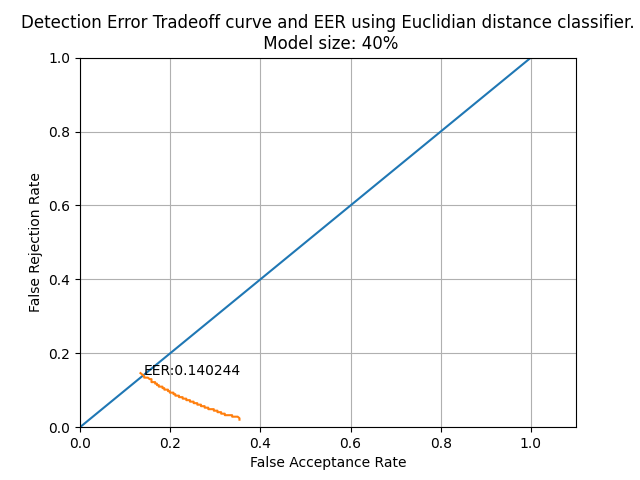
\includegraphics[width=\linewidth]{images/results/det/DET_for_classifier_Euclidian_40}
				\caption{DET curve of Euclidean distance results, model at 40\%}
				\label{fig:detforclassifiereuclidian40}
			\end{figure}
		
		\subsubsection{BARK scale with Haar \textit{wavelet} using an Euclidean distance classifier at 50\% model}
		
			\begin{table}[H]
	\newcommand{\mc}[3]{\multicolumn{#1}{#2}{#3}}
	\definecolor{tcB}{rgb}{0.447059,0.74902,0.266667}
	\definecolor{tcC}{rgb}{0,0,0}
	\definecolor{tcD}{rgb}{0,0.5,1}
	\definecolor{tcA}{rgb}{0.65098,0.65098,0.65098}
	\begin{center}
		\subfloat[Best matrix]{
			\begin{tabular}{ccc}
				% use packages: color,colortbl
				\mc{1}{l}{} & \mc{1}{>{\columncolor{tcA}}c}{\textbf{genuine}} & \mc{1}{>{\columncolor{tcA}}c}{\textbf{spoofed}}\\
				
				\mc{1}{>{\columncolor{tcA}}r}{\textbf{genuine}} & \mc{1}{>{\columncolor{tcB}}c}{\textcolor{tcC}{195}} & \mc{1}{>{\columncolor{tcD}}c}{\textcolor{tcC}{29}}\\
				
				\mc{1}{>{\columncolor{tcA}}r}{\textbf{spoofed}} & \mc{1}{>{\columncolor{tcD}}c}{\textcolor{tcC}{10}} & \mc{1}{>{\columncolor{tcB}}c}{\textcolor{tcC}{176}}
			\end{tabular}
			\label{tab:classifier_Euclidian_50_best}
		}
		\qquad
		\subfloat[Worst matrix]{
			\begin{tabular}{ccc}
				% use packages: color,colortbl
				\mc{1}{l}{} & \mc{1}{>{\columncolor{tcA}}c}{\textbf{genuine}} & \mc{1}{>{\columncolor{tcA}}c}{\textbf{spoofed}}\\
				
				\mc{1}{>{\columncolor{tcA}}r}{\textbf{genuine}} & \mc{1}{>{\columncolor{tcB}}c}{\textcolor{tcC}{193}} & \mc{1}{>{\columncolor{tcD}}c}{\textcolor{tcC}{79}}\\
				
				\mc{1}{>{\columncolor{tcA}}r}{\textbf{spoofed}} & \mc{1}{>{\columncolor{tcD}}c}{\textcolor{tcC}{12}} & \mc{1}{>{\columncolor{tcB}}c}{\textcolor{tcC}{126}}
			\end{tabular}
			\label{tab:classifier_Euclidian_50_worse}
		}
	\end{center}
	\caption{Confusion matrices for Euclidian distance classifier at 50\% model}
\end{table}
			
			\begin{figure}[!ht]
				\centering
				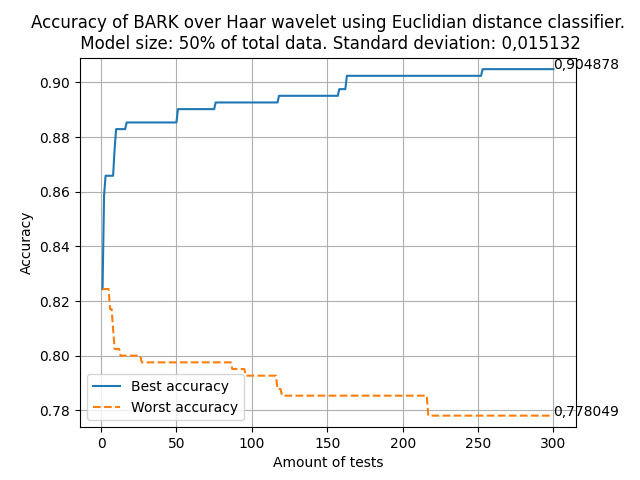
\includegraphics[width=\linewidth]{images/results/confusionMatrices/classifier_Euclidian_50}
				\caption{Accuracy \textit{X} number of tests - Euclidean distance, model at 50\%}
				\label{fig:classifiereuclidian50}
			\end{figure}
			
			\begin{figure}[!h]
				\centering
				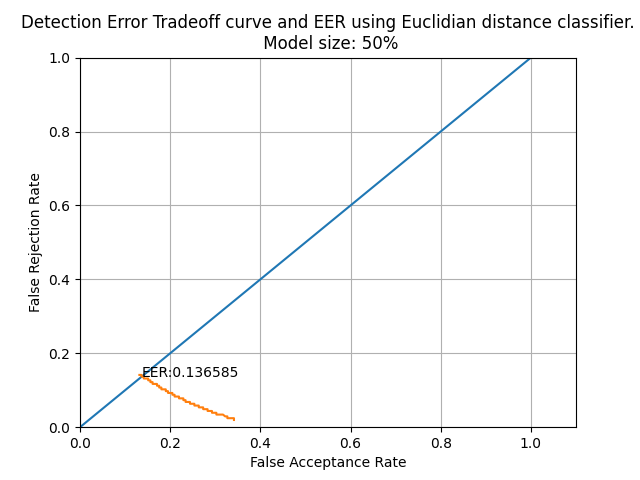
\includegraphics[width=.9\linewidth]{images/results/det/DET_for_classifier_Euclidian_50}
				\caption{DET curve of Euclidean distance results, model at 50\%}
				\label{fig:detforclassifiereuclidian50}
			\end{figure}
		
		\subsubsection{BARK scale with Haar \textit{wavelet} using an Manhattan distance classifier at 10\% model}
			
			\begin{table}[h] 					\newcommand{\mc}[3]{\multicolumn{#1}{#2}{#3}} 					\definecolor{tcB}{rgb}{0.447059,0.74902,0.266667} 					\definecolor{tcC}{rgb}{0,0,0} 					\definecolor{tcD}{rgb}{0,0.5,1} 					\definecolor{tcA}{rgb}{0.65098,0.65098,0.65098} 					\begin{center} 						\subfloat[Melhor matriz de confusão]{ 							\begin{tabular}{ccc} 								\mc{1}{l}{} & \mc{1}{>{\columncolor{tcA}}c}{\textbf{genuíno}} & \mc{1}{>{\columncolor{tcA}}c}{\textbf{falsificado}}\\ 								\mc{1}{>{\columncolor{tcA}}r}{\textbf{genuíno}} & \mc{1}{>{\columncolor{tcB}}c}{\textcolor{tcC}{365}} & \mc{1}{>{\columncolor{tcD}}c}{\textcolor{tcC}{14}}\\ 								\mc{1}{>{\columncolor{tcA}}r}{\textbf{falsificado}} & \mc{1}{>{\columncolor{tcD}}c}{\textcolor{tcC}{4}} & \mc{1}{>{\columncolor{tcB}}c}{\textcolor{tcC}{355}} 							\end{tabular} 							\label{tab:classifier_Manhattan_10_best} 						} 						\qquad 						\subfloat[Pior matriz de confusão]{ 							\begin{tabular}{ccc} 								\mc{1}{l}{} & \mc{1}{>{\columncolor{tcA}}c}{\textbf{genuíno}} & \mc{1}{>{\columncolor{tcA}}c}{\textbf{falsificado}}\\ 								\mc{1}{>{\columncolor{tcA}}r}{\textbf{genuíno}} & \mc{1}{>{\columncolor{tcB}}c}{\textcolor{tcC}{289}} & \mc{1}{>{\columncolor{tcD}}c}{\textcolor{tcC}{11}}\\ 								\mc{1}{>{\columncolor{tcA}}r}{\textbf{falsificado}} & \mc{1}{>{\columncolor{tcD}}c}{\textcolor{tcC}{80}} & \mc{1}{>{\columncolor{tcB}}c}{\textcolor{tcC}{358}} 							\end{tabular} 							\label{tab:classifier_Manhattan_10_worse} 						} 					\end{center} 					\caption{Matrizes de confusão para distância Manhattan com modelo a 10\%} 				\end{table}
			
			\begin{figure}[ht]
				\centering
				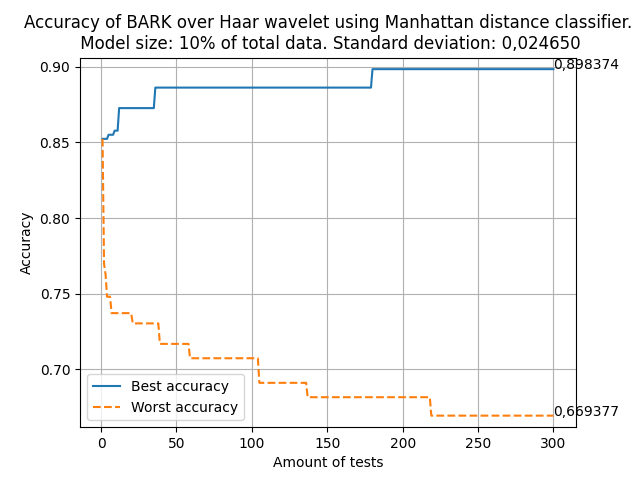
\includegraphics[width=\linewidth]{images/results/confusionMatrices/classifier_Manhattan_10.png}
				\caption{Accuracy \textit{X} number of tests - Manhattan distance, model at 10\%}
				\label{fig:classifiermanhattan10}
			\end{figure}
			
			\begin{figure}[!ht]
				\centering
				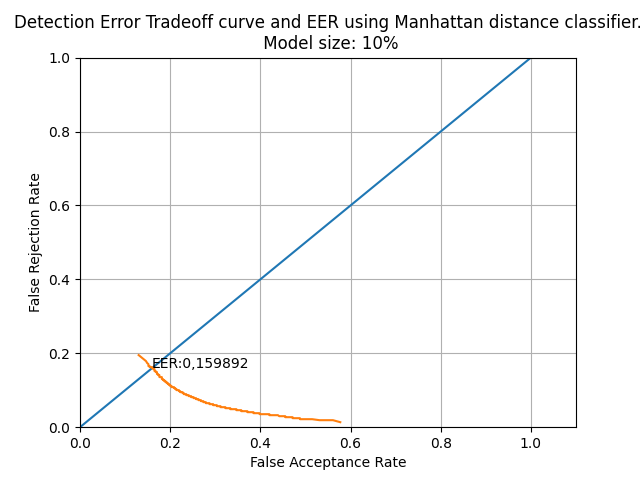
\includegraphics[width=\linewidth]{images/results/det/DET_for_classifier_Manhattan_10}
				\caption{DET curve of Manhattan distance results, model at 10\%}
				\label{fig:detforclassifiermanhattan10}
			\end{figure}
		
		\subsubsection{BARK scale with Haar \textit{wavelet} using an Manhattan distance classifier at 20\% model}
			
			\begin{table}[h]
	\newcommand{\mc}[3]{\multicolumn{#1}{#2}{#3}}
	\definecolor{tcB}{rgb}{0.447059,0.74902,0.266667}
	\definecolor{tcC}{rgb}{0,0,0}
	\definecolor{tcD}{rgb}{0,0.5,1}
	\definecolor{tcA}{rgb}{0.65098,0.65098,0.65098}
	\begin{center}
		\subfloat[Melhor matriz]{
			\begin{tabular}{ccc}
				% use packages: color,colortbl
				\mc{1}{l}{} & \mc{1}{>{\columncolor{tcA}}c}{\textbf{Verdadeiro}} & \mc{1}{>{\columncolor{tcA}}c}{\textbf{Falso}}\\
				
				\mc{1}{>{\columncolor{tcA}}r}{\textbf{Verdadeiro}} & \mc{1}{>{\columncolor{tcB}}c}{\textcolor{tcC}{308}} & \mc{1}{>{\columncolor{tcD}}c}{\textcolor{tcC}{44}}\\
				
				\mc{1}{>{\columncolor{tcA}}r}{\textbf{Falso}} & \mc{1}{>{\columncolor{tcD}}c}{\textcolor{tcC}{20}} & \mc{1}{>{\columncolor{tcB}}c}{\textcolor{tcC}{284}}
			\end{tabular}
			\label{tab:classifier_Manhattan_20_best}
		}
		\qquad
		\subfloat[Pior matriz]{
			\begin{tabular}{ccc}
				% use packages: color,colortbl
				\mc{1}{l}{} & \mc{1}{>{\columncolor{tcA}}c}{\textbf{Verdadeiro}} & \mc{1}{>{\columncolor{tcA}}c}{\textbf{Falso}}\\
				
				\mc{1}{>{\columncolor{tcA}}r}{\textbf{Verdadeiro}} & \mc{1}{>{\columncolor{tcB}}c}{\textcolor{tcC}{316}} & \mc{1}{>{\columncolor{tcD}}c}{\textcolor{tcC}{149}}\\
				
				\mc{1}{>{\columncolor{tcA}}r}{\textbf{Falso}} & \mc{1}{>{\columncolor{tcD}}c}{\textcolor{tcC}{12}} & \mc{1}{>{\columncolor{tcB}}c}{\textcolor{tcC}{179}}
			\end{tabular}
			\label{tab:classifier_Manhattan_20_worst}
		}
	\end{center}
	\caption{Matrizes de confusão para o classificador por distâncias Manhattan com o uso de 20\% da base para modelagem}
\end{table}

			
			\begin{figure}[!ht]
				\centering
				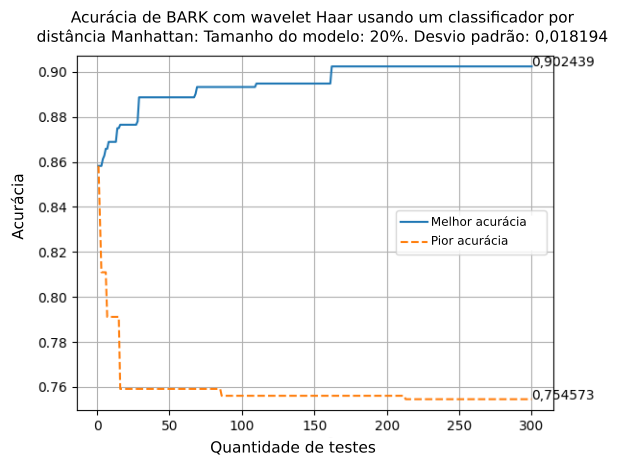
\includegraphics[width=\linewidth]{images/results/confusionMatrices/classifier_Manhattan_20.png}
				\caption{Accuracy \textit{X} number of tests - Manhattan distance, model at 20\%}
				\label{fig:classifiermanhattan20}
			\end{figure}
			
			\begin{figure}[!h]
				\centering
				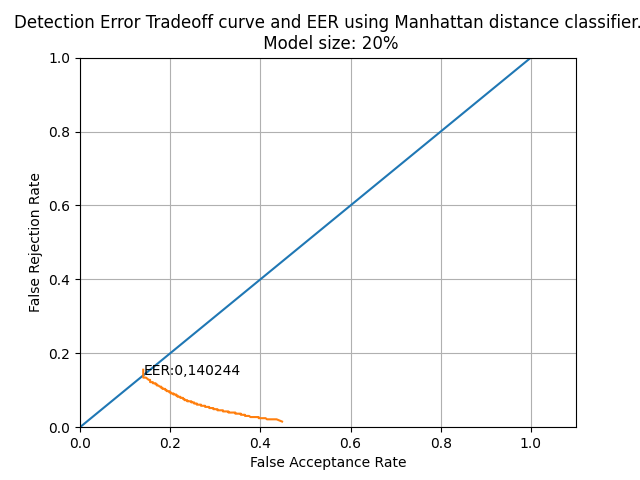
\includegraphics[width=.9\linewidth]{images/results/det/DET_for_classifier_Manhattan_20}
				\caption{DET curve of Manhattan distance results, model at 20\%}
				\label{fig:detforclassifiermanhattan20}
			\end{figure}
		
		\subsubsection{BARK scale with Haar \textit{wavelet} using an Manhattan distance classifier at 30\% model}
			
			\begin{table}[h] 					\newcommand{\mc}[3]{\multicolumn{#1}{#2}{#3}} 					\definecolor{tcB}{rgb}{0.447059,0.74902,0.266667} 					\definecolor{tcC}{rgb}{0,0,0} 					\definecolor{tcD}{rgb}{0,0.5,1} 					\definecolor{tcA}{rgb}{0.65098,0.65098,0.65098} 					\begin{center} 						\subfloat[Melhor matriz de confusão]{ 							\begin{tabular}{ccc} 								\mc{1}{l}{} & \mc{1}{>{\columncolor{tcA}}c}{\textbf{genuíno}} & \mc{1}{>{\columncolor{tcA}}c}{\textbf{falsificado}}\\ 								\mc{1}{>{\columncolor{tcA}}r}{\textbf{genuíno}} & \mc{1}{>{\columncolor{tcB}}c}{\textcolor{tcC}{281}} & \mc{1}{>{\columncolor{tcD}}c}{\textcolor{tcC}{2}}\\ 								\mc{1}{>{\columncolor{tcA}}r}{\textbf{falsificado}} & \mc{1}{>{\columncolor{tcD}}c}{\textcolor{tcC}{6}} & \mc{1}{>{\columncolor{tcB}}c}{\textcolor{tcC}{285}} 							\end{tabular} 							\label{tab:classifier_Manhattan_30_best} 						} 						\qquad 						\subfloat[Pior matriz de confusão]{ 							\begin{tabular}{ccc} 								\mc{1}{l}{} & \mc{1}{>{\columncolor{tcA}}c}{\textbf{genuíno}} & \mc{1}{>{\columncolor{tcA}}c}{\textbf{falsificado}}\\ 								\mc{1}{>{\columncolor{tcA}}r}{\textbf{genuíno}} & \mc{1}{>{\columncolor{tcB}}c}{\textcolor{tcC}{256}} & \mc{1}{>{\columncolor{tcD}}c}{\textcolor{tcC}{19}}\\ 								\mc{1}{>{\columncolor{tcA}}r}{\textbf{falsificado}} & \mc{1}{>{\columncolor{tcD}}c}{\textcolor{tcC}{31}} & \mc{1}{>{\columncolor{tcB}}c}{\textcolor{tcC}{268}} 							\end{tabular} 							\label{tab:classifier_Manhattan_30_worse} 						} 					\end{center} 					\caption{Matrizes de confusão para distância Manhattan com modelo a 30\%} 				\end{table}
			
			\begin{figure}[ht]
				\centering
				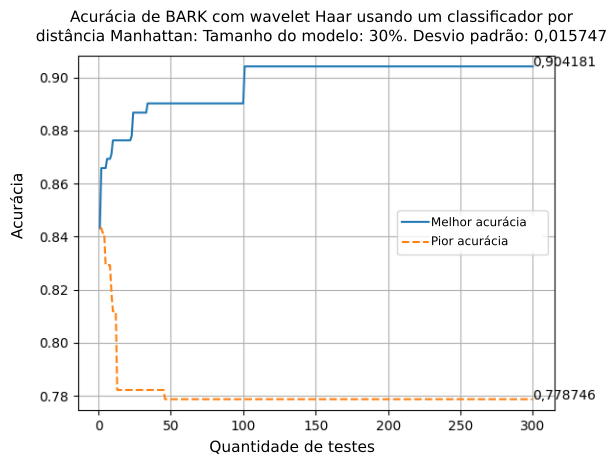
\includegraphics[width=\linewidth]{images/results/confusionMatrices/classifier_Manhattan_30.png}
				\caption{Accuracy \textit{X} number of tests - Manhattan distance, model at 30\%}
				\label{fig:classifiermanhattan30}
			\end{figure}
			
			\begin{figure}[!ht]
				\centering
				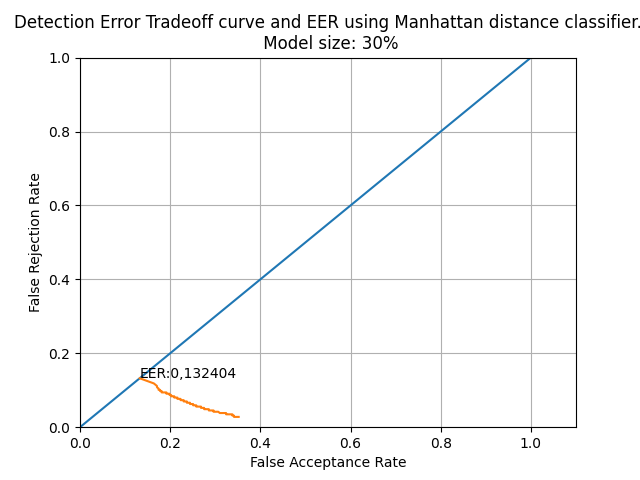
\includegraphics[width=\linewidth]{images/results/det/DET_for_classifier_Manhattan_30}
				\caption{DET curve of Manhattan distance results, model at 30\%}
				\label{fig:detforclassifiermanhattan30}
			\end{figure}
		
		\subsubsection{BARK scale with Haar \textit{wavelet} using an Manhattan distance classifier at 40\% model}
			
			\begin{table}[h] 					\newcommand{\mc}[3]{\multicolumn{#1}{#2}{#3}} 					\definecolor{tcB}{rgb}{0.447059,0.74902,0.266667} 					\definecolor{tcC}{rgb}{0,0,0} 					\definecolor{tcD}{rgb}{0,0.5,1} 					\definecolor{tcA}{rgb}{0.65098,0.65098,0.65098} 					\begin{center} 						\subfloat[Best confusion matrix]{ 							\begin{tabular}{ccc} 								\mc{1}{l}{} & \mc{1}{>{\columncolor{tcA}}c}{\textbf{genuine}} & \mc{1}{>{\columncolor{tcA}}c}{\textbf{spoofed}}\\ 								\mc{1}{>{\columncolor{tcA}}r}{\textbf{genuine}} & \mc{1}{>{\columncolor{tcB}}c}{\textcolor{tcC}{244}} & \mc{1}{>{\columncolor{tcD}}c}{\textcolor{tcC}{5}}\\ 								\mc{1}{>{\columncolor{tcA}}r}{\textbf{spoofed}} & \mc{1}{>{\columncolor{tcD}}c}{\textcolor{tcC}{2}} & \mc{1}{>{\columncolor{tcB}}c}{\textcolor{tcC}{241}} 							\end{tabular} 							\label{tab:classifier_Manhattan_40_best} 						} 						\qquad 						\subfloat[Worst confusion matrix]{ 							\begin{tabular}{ccc} 								\mc{1}{l}{} & \mc{1}{>{\columncolor{tcA}}c}{\textbf{genuine}} & \mc{1}{>{\columncolor{tcA}}c}{\textbf{spoofed}}\\ 								\mc{1}{>{\columncolor{tcA}}r}{\textbf{genuine}} & \mc{1}{>{\columncolor{tcB}}c}{\textcolor{tcC}{218}} & \mc{1}{>{\columncolor{tcD}}c}{\textcolor{tcC}{7}}\\ 								\mc{1}{>{\columncolor{tcA}}r}{\textbf{spoofed}} & \mc{1}{>{\columncolor{tcD}}c}{\textcolor{tcC}{28}} & \mc{1}{>{\columncolor{tcB}}c}{\textcolor{tcC}{239}} 							\end{tabular} 							\label{tab:classifier_Manhattan_40_worse} 						} 					\end{center} 					\caption{Confusion matrices for Manhattan distance classifier at 40\% model} 				\end{table}
			
			\begin{figure}[!ht]
				\centering
				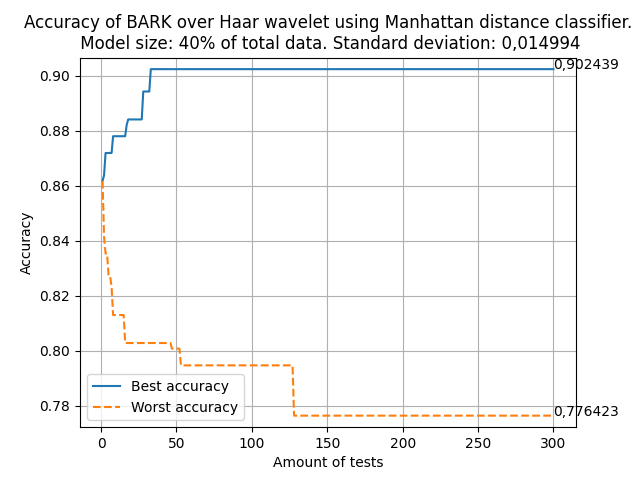
\includegraphics[width=\linewidth]{images/results/confusionMatrices/classifier_Manhattan_40.png}
				\caption{Accuracy \textit{X} number of tests - Manhattan distance, model at 40\%}
				\label{fig:classifiermanhattan40}
			\end{figure}
			
			\begin{figure}[!h]
				\centering
				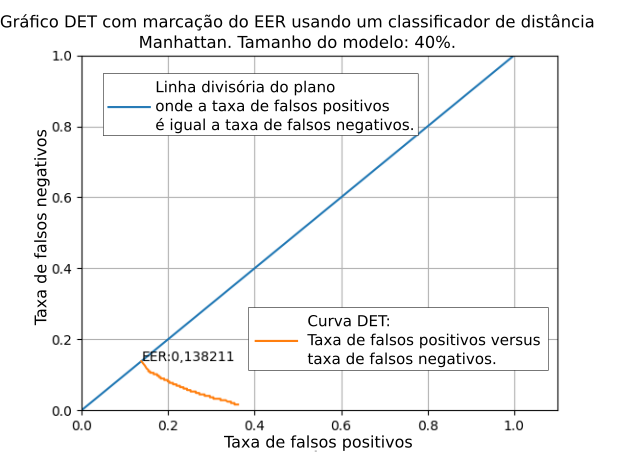
\includegraphics[width=.9\linewidth]{images/results/det/DET_for_classifier_Manhattan_40}
				\caption{DET curve of Manhattan distance results, model at 40\%}
				\label{fig:detforclassifiermanhattan40}
			\end{figure}
		
		\subsubsection{BARK scale with Haar \textit{wavelet} using an Manhattan distance classifier at 50\% model}
			
			\begin{table}[h] 					\newcommand{\mc}[3]{\multicolumn{#1}{#2}{#3}} 					\definecolor{tcB}{rgb}{0.447059,0.74902,0.266667} 					\definecolor{tcC}{rgb}{0,0,0} 					\definecolor{tcD}{rgb}{0,0.5,1} 					\definecolor{tcA}{rgb}{0.65098,0.65098,0.65098} 					\begin{center} 						\subfloat[Best confusion matrix]{ 							\begin{tabular}{ccc} 								\mc{1}{l}{} & \mc{1}{>{\columncolor{tcA}}c}{\textbf{genuine}} & \mc{1}{>{\columncolor{tcA}}c}{\textbf{spoofed}}\\ 								\mc{1}{>{\columncolor{tcA}}r}{\textbf{genuine}} & \mc{1}{>{\columncolor{tcB}}c}{\textcolor{tcC}{172}} & \mc{1}{>{\columncolor{tcD}}c}{\textcolor{tcC}{30}}\\ 								\mc{1}{>{\columncolor{tcA}}r}{\textbf{spoofed}} & \mc{1}{>{\columncolor{tcD}}c}{\textcolor{tcC}{33}} & \mc{1}{>{\columncolor{tcB}}c}{\textcolor{tcC}{175}} 							\end{tabular} 							\label{tab:classifier_Manhattan_50_best} 						} 						\qquad 						\subfloat[Worst confusion matrix]{ 							\begin{tabular}{ccc} 								\mc{1}{l}{} & \mc{1}{>{\columncolor{tcA}}c}{\textbf{genuine}} & \mc{1}{>{\columncolor{tcA}}c}{\textbf{spoofed}}\\ 								\mc{1}{>{\columncolor{tcA}}r}{\textbf{genuine}} & \mc{1}{>{\columncolor{tcB}}c}{\textcolor{tcC}{142}} & \mc{1}{>{\columncolor{tcD}}c}{\textcolor{tcC}{58}}\\ 								\mc{1}{>{\columncolor{tcA}}r}{\textbf{spoofed}} & \mc{1}{>{\columncolor{tcD}}c}{\textcolor{tcC}{63}} & \mc{1}{>{\columncolor{tcB}}c}{\textcolor{tcC}{147}} 							\end{tabular} 							\label{tab:classifier_Manhattan_50_worse} 						} 					\end{center} 					\caption{Confusion matrices for Manhattan distance classifier at 50\% model} 				\end{table}
			
			\begin{figure}[ht]
				\centering
				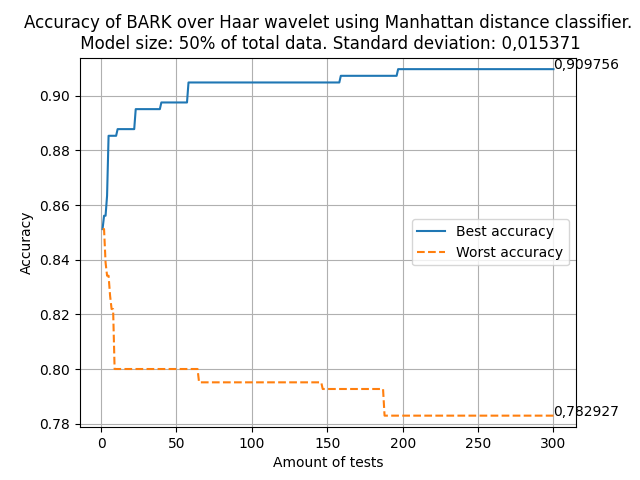
\includegraphics[width=\linewidth]{images/results/confusionMatrices/classifier_Manhattan_50.png}
				\caption{Accuracy \textit{X} number of tests - Manhattan distance, model at 50\%}
				\label{fig:classifiermanhattan50}
			\end{figure}
			
			\begin{figure}[!ht]
				\centering
				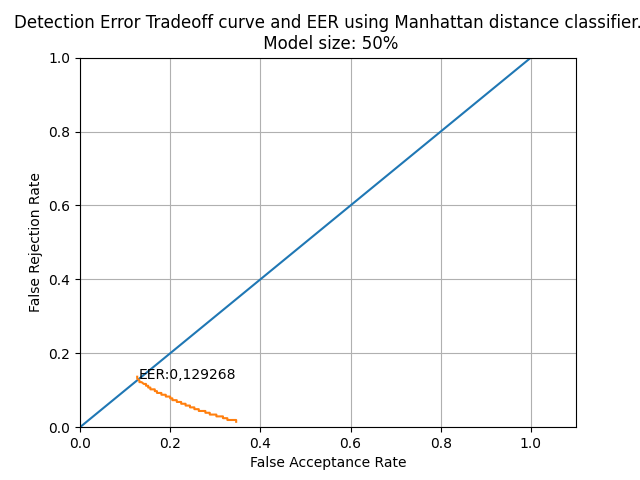
\includegraphics[width=.9\linewidth]{images/results/det/DET_for_classifier_Manhattan_50}
				\caption{DET curve of Manhattan distance results, model at 50\%}
				\label{fig:detforclassifiermanhattan50}
			\end{figure}
		
	\subsection{Synthesis}
		\par Looking at the Tables, it is noted that the \textbf{best accuracy/EERs} values are \textbf{0.904878/0.135858} and \textbf{0.909756/0.129268} for the Euclidean and Manhattan distances respectively. Thus, there is no practical difference in the metric \textit{pattern-matching} criteria used and, in addition, a relatively high level of accuracy considering the classifier algorithm simplicity.
		
	\subsection{Procedure 3}
		\label{chap:testsResults:sec:Experimento03}
		\par Novamente, considerando que o procedimento 01 apresentou, como melhor resultado, a combinação \textbf{Haar + Bark}, o objetivo deste procedimento é constatar a \textbf{máxima acurácia e mínimo EER} que se consegue atingir com uma SVM. Os resultados, obedecendo os mesmo moldes do procedimento anterior, constam na Tabela \ref{tab:experiment03Results}.
		
		\par Again, considering that procedure 01 presented, as best result, the combination \textbf{Haar Bark}, the objective of this procedure is to verify the \textbf{maximum accuracy and minimum EER} that can be achieved with an SVM. The results, following the same pattern as the previous procedure, are shown in the Table \ref{tab:experiment03Results}.
		
		
		\par More levels of detail can be found in the Tables
		 \ref{tab:classifier_SVM_10_best}, \ref{tab:classifier_SVM_10_worse}, \ref{tab:classifier_SVM_20_best}, \ref{tab:classifier_SVM_20_worse}, \ref{tab:classifier_SVM_30_best}, \ref{tab:classifier_SVM_30_worse}, \ref{tab:classifier_SVM_40_best}, \ref{tab:classifier_SVM_40_worse}, \ref{tab:classifier_SVM_50_best} e \ref{tab:classifier_SVM_50_worse}, in addition to their respective graphs are in Figures \ref{fig:classifiersvm10}, \ref{fig:classifiersvm20}, \ref{fig:classifiersvm30}, \ref{fig:classifiersvm40} e \ref{fig:classifiersvm50}.
		
		\begin{table}[H]
	\newcommand{\mc}[3]{\multicolumn{#1}{#2}{#3}}
	\definecolor{tcA}{rgb}{0.65098,0.65098,0.65098}
	\definecolor{tcB}{rgb}{0.447059,0.74902,0.266667}
	\begin{center}
		\caption{Resultados da abordagem com SVM}
		\begin{tabular}{|p{0.15\linewidth}|p{0.11\linewidth}|p{0.11\linewidth}|p{0.11\linewidth}|p{0.14\linewidth}|p{0.14\linewidth}|}\hline
			% use packages: color,colortbl
			\rowcolor{tcA}
			\centering\textbf{$M$} & \centering\textbf{Acurácia mínima} & \centering\textbf{Acurácia máxima} & \centering\textbf{Média das acurácias} & \centering\textbf{Desvio padrão da acurácia} & \begin{center}\textbf{EER}\end{center}\\\hline
			
			\rowcolor{tcB}
			% Loads data from tables/results/paraconsistentPlane/distParacomFrom10.csv
			\csvreader[
			late after line=\\\hline\rowcolor{tcB},%
			separator=comma,
			]{tables/results/experiment02ResultsSVM.csv}{1=\eme,2=\minAccu,3=\maxAccu,4=\meanAccu,5=\stdDev,6=\eer}{\centering\eme\% & \centering\StrSubstitute[0]{\minAccu}{.}{,} & \centering\StrSubstitute[0]{\maxAccu}{.}{,} & \centering\StrSubstitute[0]{\meanAccu}{.}{,} & \centering\StrSubstitute[0]{\stdDev}{.}{,} & \StrSubstitute[0]{\eer}{.}{,}}
			
		\end{tabular}
		\label{tab:experiment03Results}
		\\Fonte: Elaborado pelo autor, 2021.
	\end{center}
\end{table}
		
		\subsubsection{BARK scale with Haar \textit{wavelet} using a SVM classifier at 10\% model}
			
			\begin{table}[h]
\newcommand{\mc}[3]{\multicolumn{#1}{#2}{#3}}
\definecolor{tcB}{rgb}{0.447059,0.74902,0.266667}
\definecolor{tcC}{rgb}{0,0,0}
\definecolor{tcD}{rgb}{0,0.4,0.701961}
\definecolor{tcA}{rgb}{0.65098,0.65098,0.65098}
\begin{center}
	\begin{tabular}{ccc}
		% use packages: color,colortbl
		\mc{1}{l}{} & \mc{1}{>{\columncolor{tcA}}c}{\textbf{Verdadeiro}} & \mc{1}{>{\columncolor{tcA}}c}{\textbf{Falso}}\\

		\mc{1}{>{\columncolor{tcA}}r}{\textbf{Verdadeiro}} & \mc{1}{>{\columncolor{tcB}}c}{\textcolor{tcC}{339}} & \mc{1}{>{\columncolor{tcD}}c}{\textcolor{tcC}{24}}\\

		\mc{1}{>{\columncolor{tcA}}r}{\textbf{Falso}} & \mc{1}{>{\columncolor{tcD}}c}{\textcolor{tcC}{30}} & \mc{1}{>{\columncolor{tcB}}c}{\textcolor{tcC}{345}}
	\end{tabular}
	\caption{Melhor tabela de confusão para classificador SVM 10\%}
	\label{tab:classifier_SVM_10_best}
\end{center}
\end{table}

\begin{table}[h]
	\newcommand{\mc}[3]{\multicolumn{#1}{#2}{#3}}
	\definecolor{tcB}{rgb}{0.447059,0.74902,0.266667}
	\definecolor{tcC}{rgb}{0,0,0}
	\definecolor{tcD}{rgb}{0,0.4,0.701961}
	\definecolor{tcA}{rgb}{0.65098,0.65098,0.65098}
	\begin{center}
		\begin{tabular}{ccc}
			% use packages: color,colortbl
			\mc{1}{l}{} & \mc{1}{>{\columncolor{tcA}}c}{\textbf{Verdadeiro}} & \mc{1}{>{\columncolor{tcA}}c}{\textbf{Falso}}\\
			
			\mc{1}{>{\columncolor{tcA}}r}{\textbf{Verdadeiro}} & \mc{1}{>{\columncolor{tcB}}c}{\textcolor{tcC}{329}} & \mc{1}{>{\columncolor{tcD}}c}{\textcolor{tcC}{93}}\\
			
			\mc{1}{>{\columncolor{tcA}}r}{\textbf{Falso}} & \mc{1}{>{\columncolor{tcD}}c}{\textcolor{tcC}{40}} & \mc{1}{>{\columncolor{tcB}}c}{\textcolor{tcC}{276}}
		\end{tabular}
		\caption{Pior tabela de confusão para classificador SVM 10\%}
		\label{tab:classifier_SVM_10_worse}
	\end{center}
\end{table}

			
			\begin{figure}[H]
				\centering
				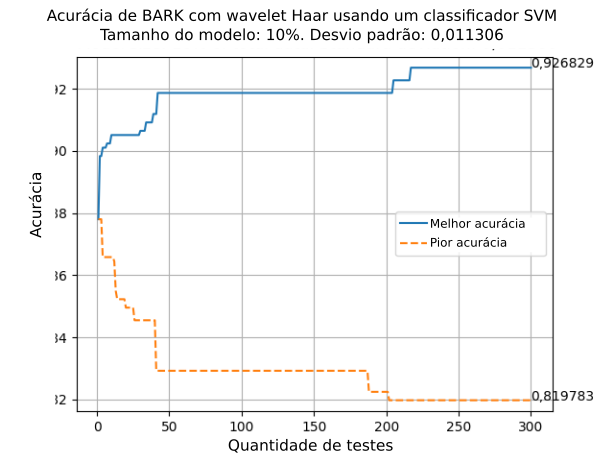
\includegraphics[width=.8\linewidth]{images/results/confusionMatrices/classifier_SVM_10.png}
				\caption{Accuracy \textit{X} number of tests - SVM, model at 10\%}
				\label{fig:classifiersvm10}
			\end{figure}
			
			\begin{figure}[H]
				\centering
				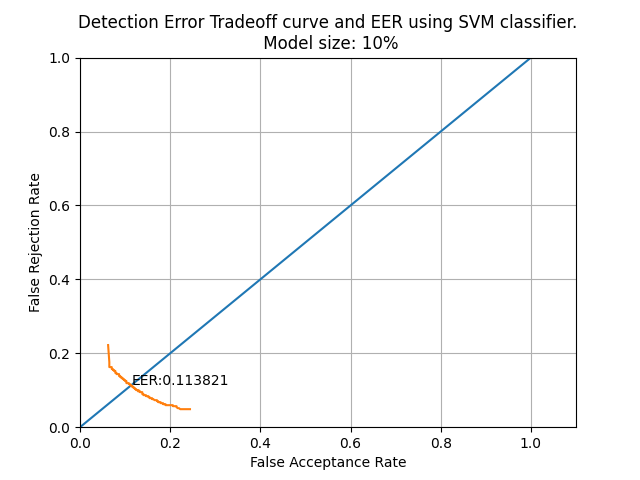
\includegraphics[width=.9\linewidth]{images/results/det/DET_SVM_10}
				\caption{DET curve of SVM results, model at 10\%}
				\label{fig:detsvm10}
			\end{figure}
		
		\subsubsection{BARK scale with Haar \textit{wavelet} using a SVM classifier at 20\% model}
			
			\begin{table}[h] 					\newcommand{\mc}[3]{\multicolumn{#1}{#2}{#3}} 					\definecolor{tcB}{rgb}{0.447059,0.74902,0.266667} 					\definecolor{tcC}{rgb}{0,0,0} 					\definecolor{tcD}{rgb}{0,0.5,1} 					\definecolor{tcA}{rgb}{0.65098,0.65098,0.65098} 					\begin{center} 						\subfloat[Best confusion matrix]{ 							\begin{tabular}{ccc} 								\mc{1}{l}{} & \mc{1}{>{\columncolor{tcA}}c}{\textbf{genuine}} & \mc{1}{>{\columncolor{tcA}}c}{\textbf{spoofed}}\\ 								\mc{1}{>{\columncolor{tcA}}r}{\textbf{genuine}} & \mc{1}{>{\columncolor{tcB}}c}{\textcolor{tcC}{306}} & \mc{1}{>{\columncolor{tcD}}c}{\textcolor{tcC}{29}}\\ 								\mc{1}{>{\columncolor{tcA}}r}{\textbf{spoofed}} & \mc{1}{>{\columncolor{tcD}}c}{\textcolor{tcC}{22}} & \mc{1}{>{\columncolor{tcB}}c}{\textcolor{tcC}{299}} 							\end{tabular} 							\label{tab:classifier_Euclidian_10_best} 						} 						\qquad 						\subfloat[Worst confusion matrix]{ 							\begin{tabular}{ccc} 								\mc{1}{l}{} & \mc{1}{>{\columncolor{tcA}}c}{\textbf{genuine}} & \mc{1}{>{\columncolor{tcA}}c}{\textbf{spoofed}}\\ 								\mc{1}{>{\columncolor{tcA}}r}{\textbf{genuine}} & \mc{1}{>{\columncolor{tcB}}c}{\textcolor{tcC}{255}} & \mc{1}{>{\columncolor{tcD}}c}{\textcolor{tcC}{56}}\\ 								\mc{1}{>{\columncolor{tcA}}r}{\textbf{spoofed}} & \mc{1}{>{\columncolor{tcD}}c}{\textcolor{tcC}{73}} & \mc{1}{>{\columncolor{tcB}}c}{\textcolor{tcC}{272}} 							\end{tabular} 							\label{tab:classifier_Euclidian_10_worse} 						} 					\end{center} 					\caption{Confusion matrices for SVM classifier at 20\% model} 				\end{table}
			
			\begin{figure}[h]
				\centering
				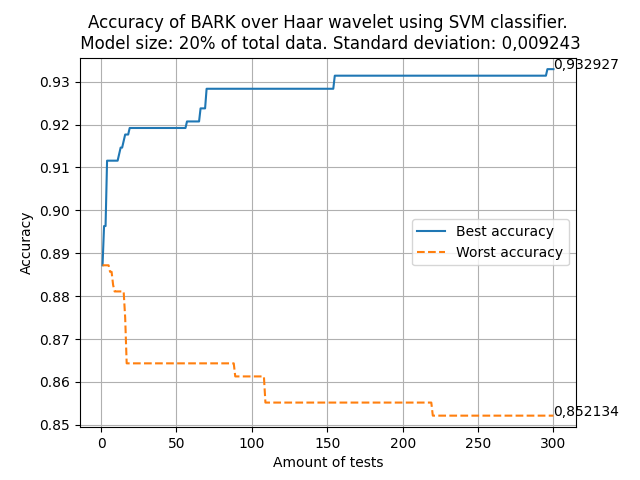
\includegraphics[width=.95\linewidth]{images/results/confusionMatrices/classifier_SVM_20.png}
				\caption{Accuracy \textit{X} number of tests - SVM, model at 20\%}
				\label{fig:classifiersvm20}
			\end{figure}
			
			\begin{figure}[h]
				\centering
				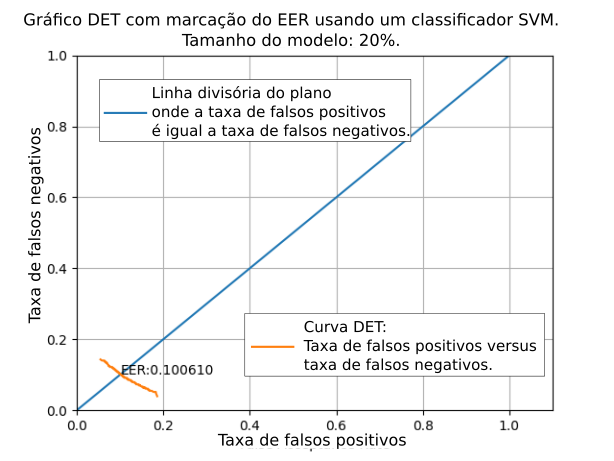
\includegraphics[width=.9\linewidth]{images/results/det/DET_SVM_20}
				\caption{DET curve of SVM results, model at 20\%}
				\label{fig:detsvm20}
			\end{figure}
		
		\subsubsection{BARK scale with Haar \textit{wavelet} using a SVM classifier at 30\% model}
			\begin{table}[h] 					\newcommand{\mc}[3]{\multicolumn{#1}{#2}{#3}} 					\definecolor{tcB}{rgb}{0.447059,0.74902,0.266667} 					\definecolor{tcC}{rgb}{0,0,0} 					\definecolor{tcD}{rgb}{0,0.5,1} 					\definecolor{tcA}{rgb}{0.65098,0.65098,0.65098} 					\begin{center} 						\subfloat[Best confusion matrix]{ 							\begin{tabular}{ccc} 								\mc{1}{l}{} & \mc{1}{>{\columncolor{tcA}}c}{\textbf{genuine}} & \mc{1}{>{\columncolor{tcA}}c}{\textbf{spoofed}}\\ 								\mc{1}{>{\columncolor{tcA}}r}{\textbf{genuine}} & \mc{1}{>{\columncolor{tcB}}c}{\textcolor{tcC}{272}} & \mc{1}{>{\columncolor{tcD}}c}{\textcolor{tcC}{27}}\\ 								\mc{1}{>{\columncolor{tcA}}r}{\textbf{spoofed}} & \mc{1}{>{\columncolor{tcD}}c}{\textcolor{tcC}{15}} & \mc{1}{>{\columncolor{tcB}}c}{\textcolor{tcC}{260}} 							\end{tabular} 							\label{tab:classifier_Euclidian_10_best} 						} 						\qquad 						\subfloat[Worst confusion matrix]{ 							\begin{tabular}{ccc} 								\mc{1}{l}{} & \mc{1}{>{\columncolor{tcA}}c}{\textbf{genuine}} & \mc{1}{>{\columncolor{tcA}}c}{\textbf{spoofed}}\\ 								\mc{1}{>{\columncolor{tcA}}r}{\textbf{genuine}} & \mc{1}{>{\columncolor{tcB}}c}{\textcolor{tcC}{233}} & \mc{1}{>{\columncolor{tcD}}c}{\textcolor{tcC}{39}}\\ 								\mc{1}{>{\columncolor{tcA}}r}{\textbf{spoofed}} & \mc{1}{>{\columncolor{tcD}}c}{\textcolor{tcC}{54}} & \mc{1}{>{\columncolor{tcB}}c}{\textcolor{tcC}{248}} 							\end{tabular} 							\label{tab:classifier_Euclidian_10_worse} 						} 					\end{center} 					\caption{Confusion matrices for SVM classifier at 30\% model} 				\end{table}
			
			\begin{figure}[ht]
				\centering
				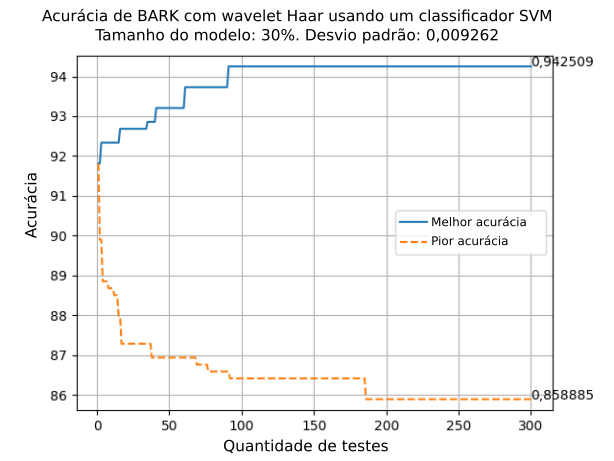
\includegraphics[width=\linewidth]{images/results/confusionMatrices/classifier_SVM_30.png}
				\caption{Accuracy \textit{X} number of tests - SVM, model at 30\%}
				\label{fig:classifiersvm30}
			\end{figure}
			
			\begin{figure}[h]
				\centering
				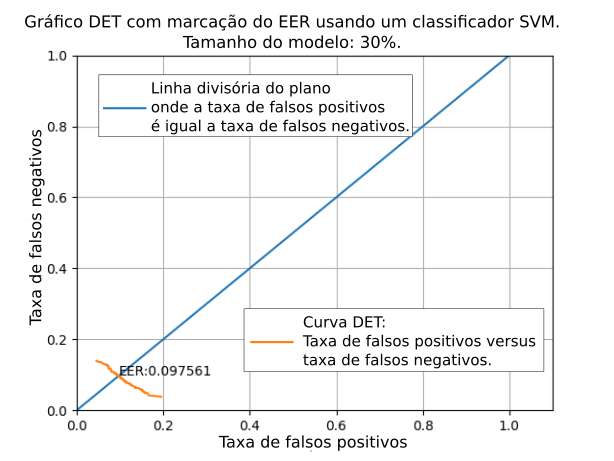
\includegraphics[width=\linewidth]{images/results/det/DET_SVM_30}
				\caption{DET curve of SVM results, model at 20\%}
				\label{fig:detsvm30}
			\end{figure}
		
		\subsubsection{BARK scale with Haar \textit{wavelet} using a SVM classifier at 40\% model}
			\begin{table}[h]
\newcommand{\mc}[3]{\multicolumn{#1}{#2}{#3}}
\definecolor{tcB}{rgb}{0.447059,0.74902,0.266667}
\definecolor{tcC}{rgb}{0,0,0}
\definecolor{tcD}{rgb}{0,0.5,1}
\definecolor{tcA}{rgb}{0.65098,0.65098,0.65098}
\begin{center}
	\begin{tabular}{ccc}
		% use packages: color,colortbl
		\mc{1}{l}{} & \mc{1}{>{\columncolor{tcA}}c}{\textbf{Verdadeiro}} & \mc{1}{>{\columncolor{tcA}}c}{\textbf{Falso}}\\

		\mc{1}{>{\columncolor{tcA}}r}{\textbf{Verdadeiro}} & \mc{1}{>{\columncolor{tcB}}c}{\textcolor{tcC}{234}} & \mc{1}{>{\columncolor{tcD}}c}{\textcolor{tcC}{14}}\\

		\mc{1}{>{\columncolor{tcA}}r}{\textbf{Falso}} & \mc{1}{>{\columncolor{tcD}}c}{\textcolor{tcC}{12}} & \mc{1}{>{\columncolor{tcB}}c}{\textcolor{tcC}{232}}
	\end{tabular}
	\caption{Melhor tabela de confusão para classificador SVM 40\%}
	\label{tab:classifier_SVM_40_best}
\end{center}
\end{table}

\begin{table}[h]
	\newcommand{\mc}[3]{\multicolumn{#1}{#2}{#3}}
	\definecolor{tcB}{rgb}{0.447059,0.74902,0.266667}
	\definecolor{tcC}{rgb}{0,0,0}
	\definecolor{tcD}{rgb}{0,0.5,1}
	\definecolor{tcA}{rgb}{0.65098,0.65098,0.65098}
	\begin{center}
		\begin{tabular}{ccc}
			% use packages: color,colortbl
			\mc{1}{l}{} & \mc{1}{>{\columncolor{tcA}}c}{\textbf{Verdadeiro}} & \mc{1}{>{\columncolor{tcA}}c}{\textbf{Falso}}\\
			
			\mc{1}{>{\columncolor{tcA}}r}{\textbf{Verdadeiro}} & \mc{1}{>{\columncolor{tcB}}c}{\textcolor{tcC}{216}} & \mc{1}{>{\columncolor{tcD}}c}{\textcolor{tcC}{37}}\\
			
			\mc{1}{>{\columncolor{tcA}}r}{\textbf{Falso}} & \mc{1}{>{\columncolor{tcD}}c}{\textcolor{tcC}{30}} & \mc{1}{>{\columncolor{tcB}}c}{\textcolor{tcC}{209}}
		\end{tabular}
		\caption{Pior tabela de confusão para classificador SVM 40\%}
		\label{tab:classifier_SVM_40_worse}
	\end{center}
\end{table}

			
			\begin{figure}[ht]
				\centering
				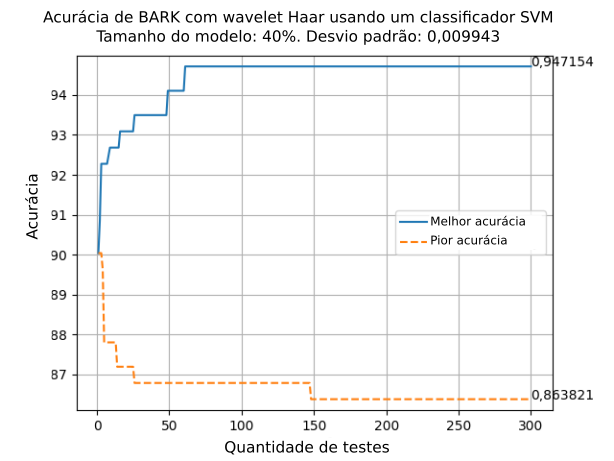
\includegraphics[width=.95\linewidth]{images/results/confusionMatrices/classifier_SVM_40.png}
				\caption{Accuracy \textit{X} number of tests - SVM, model at 40\%}
				\label{fig:classifiersvm40}
			\end{figure}
			
			\begin{figure}[!h]
				\centering
				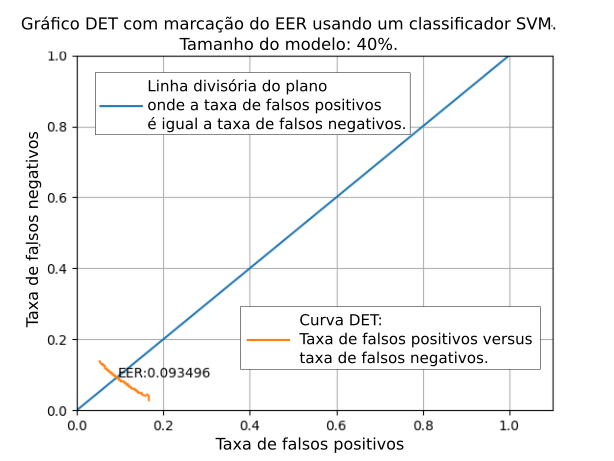
\includegraphics[width=.9\linewidth]{images/results/det/DET_SVM_40}
				\caption{DET curve of SVM results, model at 40\%}
				\label{fig:detsvm40}
			\end{figure}
		
		\subsubsection{BARK scale with Haar \textit{wavelet} using a SVM classifier at 50\% model}
			
			\begin{table}[h] 					\newcommand{\mc}[3]{\multicolumn{#1}{#2}{#3}} 					\definecolor{tcB}{rgb}{0.447059,0.74902,0.266667} 					\definecolor{tcC}{rgb}{0,0,0} 					\definecolor{tcD}{rgb}{0,0.5,1} 					\definecolor{tcA}{rgb}{0.65098,0.65098,0.65098} 					\begin{center} 						\subfloat[Best confusion matrix]{ 							\begin{tabular}{ccc} 								\mc{1}{l}{} & \mc{1}{>{\columncolor{tcA}}c}{\textbf{genuine}} & \mc{1}{>{\columncolor{tcA}}c}{\textbf{spoofed}}\\ 								\mc{1}{>{\columncolor{tcA}}r}{\textbf{genuine}} & \mc{1}{>{\columncolor{tcB}}c}{\textcolor{tcC}{205}} & \mc{1}{>{\columncolor{tcD}}c}{\textcolor{tcC}{1}}\\ 								\mc{1}{>{\columncolor{tcA}}r}{\textbf{spoofed}} & \mc{1}{>{\columncolor{tcD}}c}{\textcolor{tcC}{0}} & \mc{1}{>{\columncolor{tcB}}c}{\textcolor{tcC}{204}} 							\end{tabular} 							\label{tab:classifier_SVM_50_best} 						} 						\qquad 						\subfloat[Worst confusion matrix]{ 							\begin{tabular}{ccc} 								\mc{1}{l}{} & \mc{1}{>{\columncolor{tcA}}c}{\textbf{genuine}} & \mc{1}{>{\columncolor{tcA}}c}{\textbf{spoofed}}\\ 								\mc{1}{>{\columncolor{tcA}}r}{\textbf{genuine}} & \mc{1}{>{\columncolor{tcB}}c}{\textcolor{tcC}{196}} & \mc{1}{>{\columncolor{tcD}}c}{\textcolor{tcC}{17}}\\ 								\mc{1}{>{\columncolor{tcA}}r}{\textbf{spoofed}} & \mc{1}{>{\columncolor{tcD}}c}{\textcolor{tcC}{9}} & \mc{1}{>{\columncolor{tcB}}c}{\textcolor{tcC}{188}} 							\end{tabular} 							\label{tab:classifier_SVM_50_worse} 						} 					\end{center} 					\caption{Confusion matrices for SVM distance classifier at 50\% model} 				\end{table}
			
			\begin{figure}[!h]
				\centering
				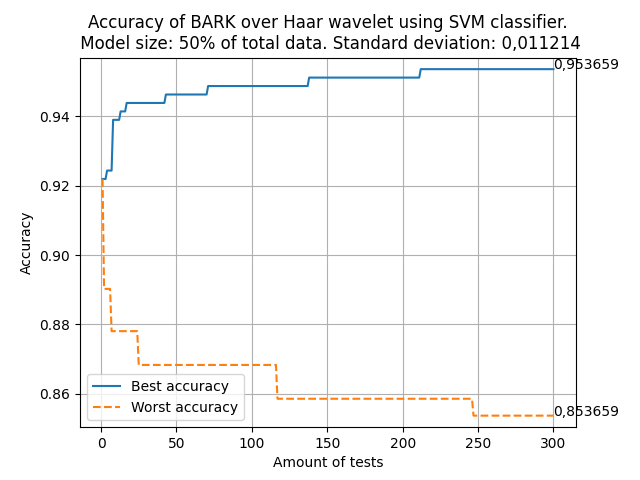
\includegraphics[width=\linewidth]{images/results/confusionMatrices/classifier_SVM_50.png}
				\caption{Accuracy \textit{X} number of tests - SVM, model at 50\%}
				\label{fig:classifiersvm50}
			\end{figure}
			
			\begin{figure}[!h]
				\centering
				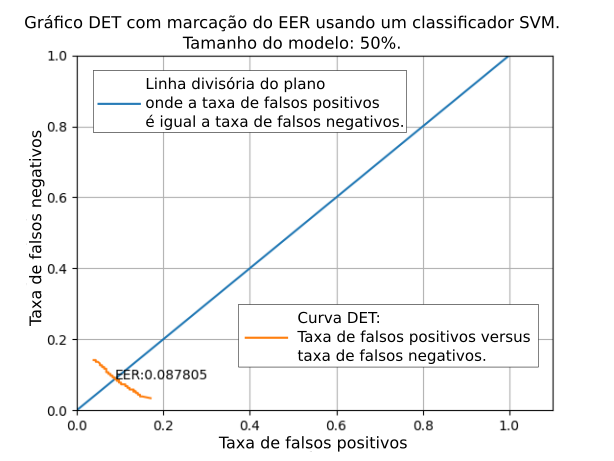
\includegraphics[width=.9\linewidth]{images/results/det/DET_SVM_50}
				\caption{DET curve of SVM results, model at 50\%}
				\label{fig:detsvm50}
			\end{figure}
		
	\subsection{Synthesis}
		\par In short, it is clear that the \textbf{best accuracy/EER} obtained was \textbf{0.953659/0.087805} with the use of SVM and 50\% of the database signal to train it, consistent with the expectations. In such a case, the respective confusion matrix reveals a minimum amount of false-genuine and false-rewritten, consistent with the related works.
		
		
	\subsection{Complementary Tests}
		\label{chap:testsResults:sec:Experimento05}
		
		\par The Figures \ref{fig:livehaarbark} and \ref{fig:spoofinghaarbark} contains, as a complement, the spreading values of the feature vectors in the \textit{wavelet-packet} Haar Bark scale. Notably, compared to Figures \ref{fig:livehaarmel} and \ref{fig:spoofinghaarmel}, the \textbf{spread of the values is much greater on the Mel} scale. This difference in data distribution also occurs in the \textit{wavelet-packet} daubechies 42 Bark combinations, as shown in Figures \ref{fig:livedaub42bark} and \ref{fig:spoofingdaub42bark}, in addition to \textit{wavelet-packet} daubechies 54 Honey, as per Figures \ref{fig:livedaub54mel} and \ref{fig:spoofingdaub54mel}.
		
		\par For comparison purposes, the graphs were placed on the same scale on the amplitude axis (vertical).
		
		\begin{figure}[!h]
			\centering
			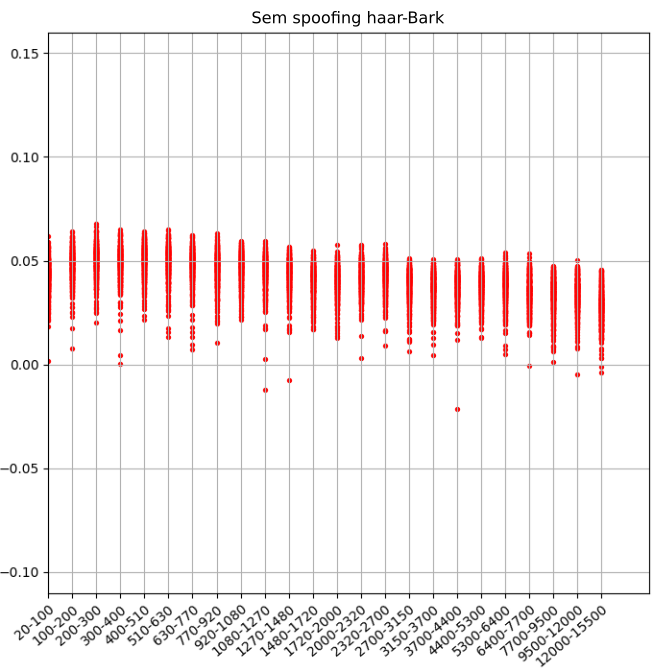
\includegraphics[width=.70\linewidth, height=.68\linewidth]{images/results/barkVersusMel/liveHaarBark}
			\caption{Scattering of feature vectors without \textit{voice spoofing} with \textit{wavelet haar} scale \textit {BARK}}
			\label{fig:livehaarbark}
		\end{figure}
		
		\begin{figure}[!h]
			\centering
			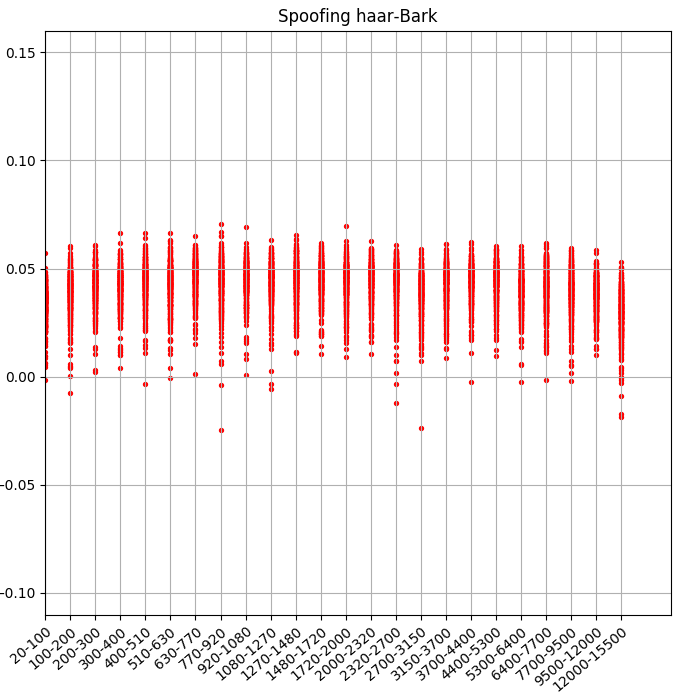
\includegraphics[width=.70\linewidth, height=.68\linewidth]{images/results/barkVersusMel/spoofingHaarBark}
			\caption{Scattering of feature vectors for \textit{voice spoofing} with \textit{wavelet haar} scale \textit{BARK}}
			\label{fig:spoofinghaarbark}
		\end{figure}
		
		\begin{figure}[!h]
			\centering
			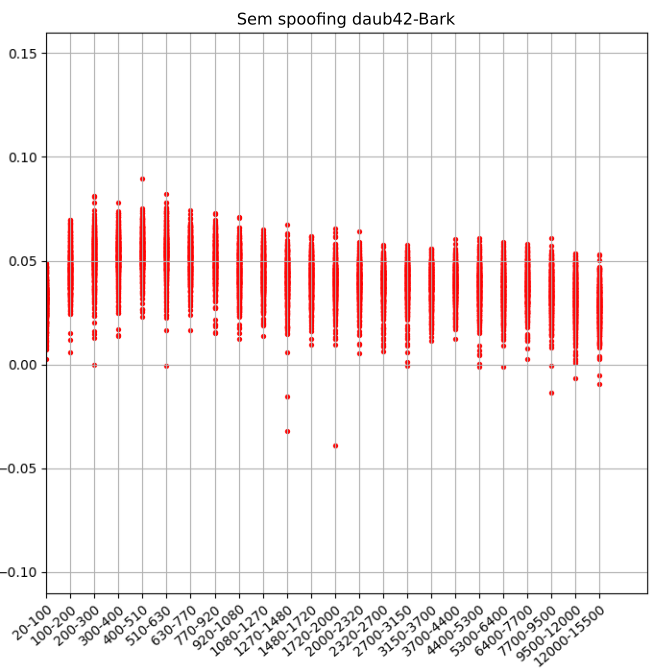
\includegraphics[width=.70\linewidth, height=.68\linewidth]{images/results/barkVersusMel/liveDaub42Bark}
			\caption{Scattering of feature vectors without \textit{voice spoofing} with \textit{wavelet daubechies 42} scale \textit{BARK}}
			\label{fig:livedaub42bark}
		\end{figure}
		
		\begin{figure}[!h]
			\centering
			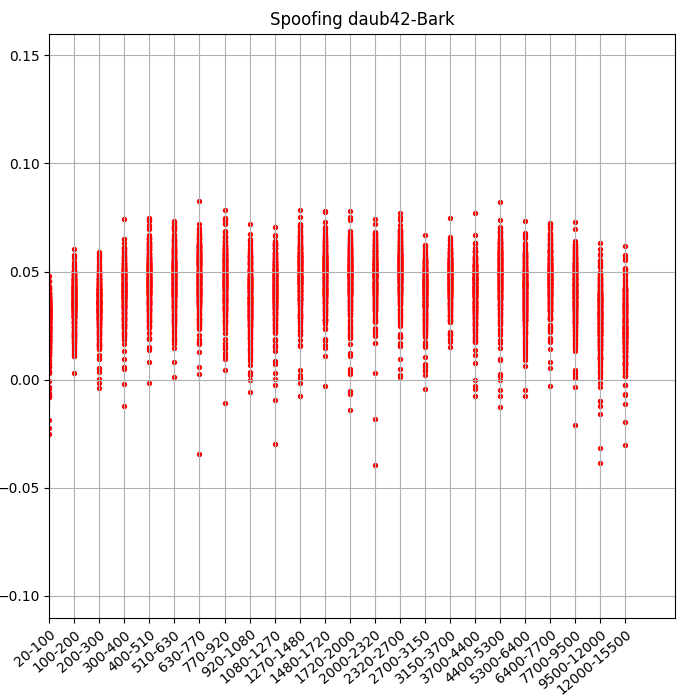
\includegraphics[width=.70\linewidth, height=.68\linewidth]{images/results/barkVersusMel/spoofingDaub42Bark}
			\caption{Scattering of feature vectors for \textit{voice spoofing} with \textit{wavelet daubechies 42} scale \textit{BARK}}
			\label{fig:spoofingdaub42bark}
		\end{figure}
		
		\begin{figure}[!h]
			\centering
			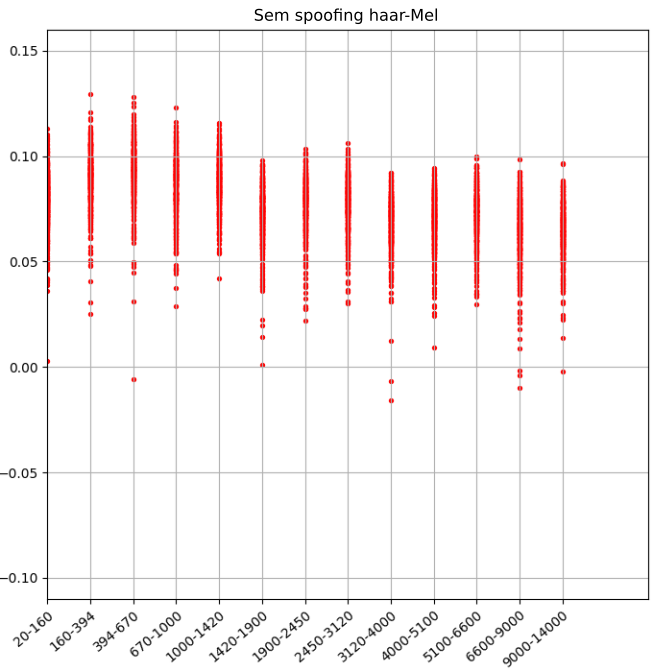
\includegraphics[width=.70\linewidth, height=.68\linewidth]{images/results/barkVersusMel/liveHaarMel}
			\caption{Scattering of feature vectors without \textit{voice spoofing} with \textit{wavelet haar} scale \textit{MEL}}
			\label{fig:livehaarmel}
		\end{figure}
		
		\begin{figure}[!h]
			\centering
			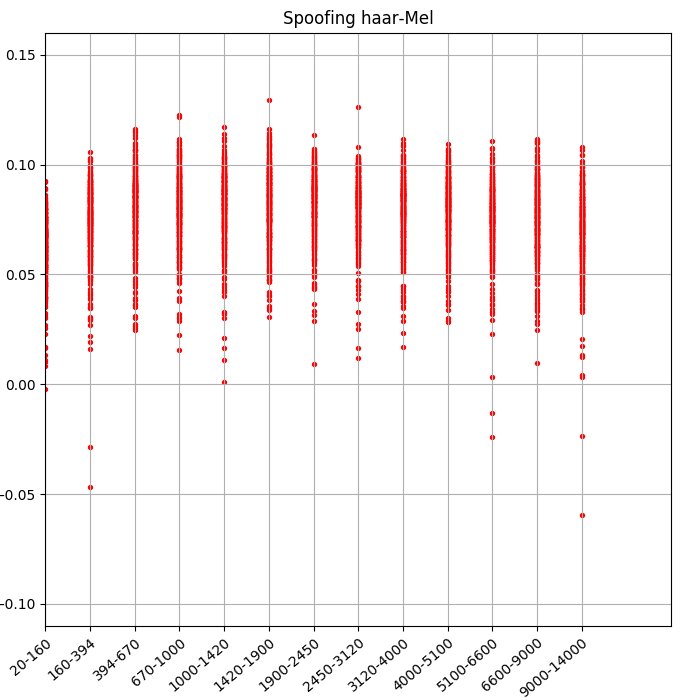
\includegraphics[width=.70\linewidth, height=.68\linewidth]{images/results/barkVersusMel/spoofingHaarMel}
			\caption{Scattering of feature vectors for \textit{voice spoofing} with \textit{wavelet haar} scale \textit{MEL}}
			\label{fig:spoofinghaarmel}
		\end{figure}
		
		\begin{figure}[!h]
			\centering
			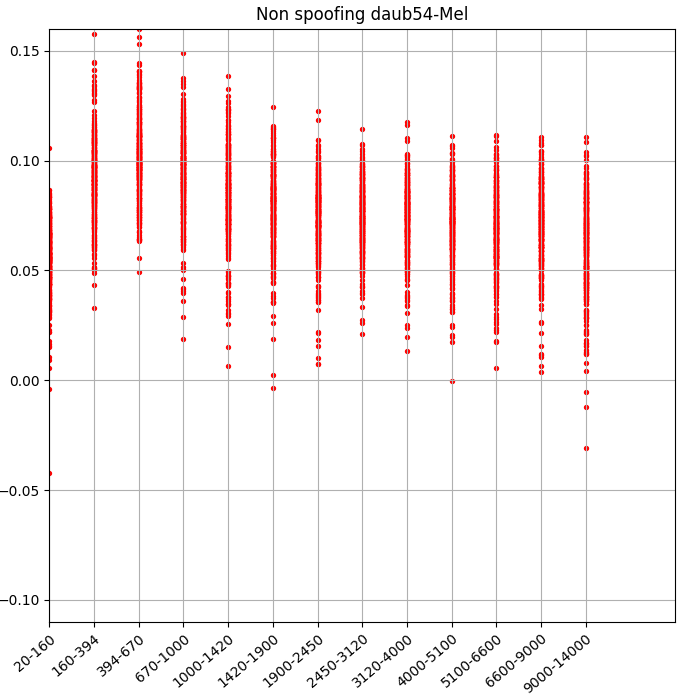
\includegraphics[width=.70\linewidth, height=.68\linewidth]{images/results/barkVersusMel/liveDaub54Mel}
			\caption{Scattering of feature vectors without \textit{voice spoofing} with \textit{wavelet daubechies 54} scale \textit{MEL}}
			\label{fig:livedaub54mel}
		\end{figure}
		
		\begin{figure}[!h]
			\centering
			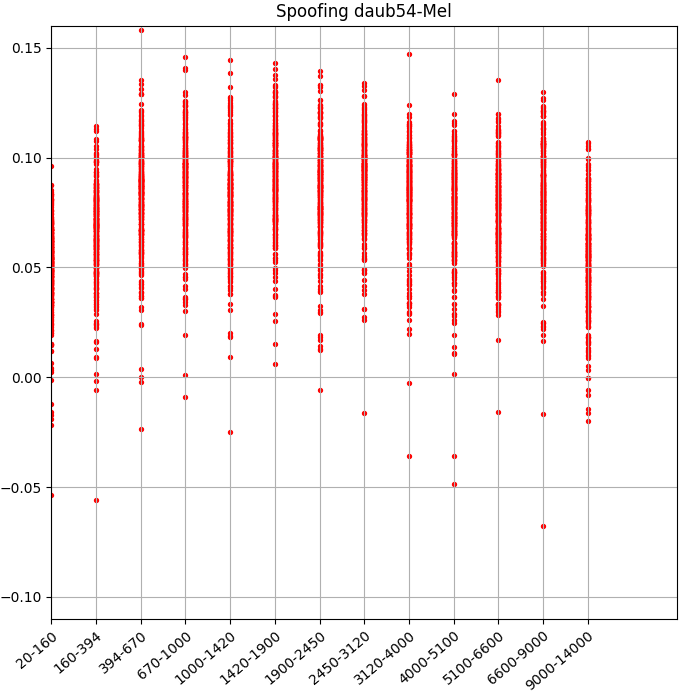
\includegraphics[width=.70\linewidth, height=.68\linewidth]{images/results/barkVersusMel/spoofingDaub54Mel}
			\caption{Scattering of feature vectors for \textit{voice spoofing} with \textit{wavelet daubechies 54} scale \textit{MEL}}
			\label{fig:spoofingdaub54mel}
		\end{figure}